%%% This is an example file for the Auburn University style options
%%%       aums.sty (Masters Thesis)
%%%       auphd.sty (Ph.D. Dissertation)
%%%       auhonors.sty (Honors Scholar)

%%%To use it, please edit the necessary options, title, author, date, year, keywords, advisor, professor, etc. 

\documentclass[12pt]{report}
\usepackage{aums}       % For Master's papers
\usepackage{ulem}       % underlining on style-page; see \normalem below
\usepackage{url}
\usepackage{tikz}
\usepackage{pgf}
\usepackage{graphicx}
\usepackage{array}
\usepackage{colortbl}
%%%%%Format rules: Normal margins are 1 in. If you need to print with 1.5in margins, uncomment the line below
%\oddsidemargin0.5in \textwidth6in

%% If you do not need a List of Abbreviations, then comment out the lines below and the \printnomenclature line.
%%for List of Abbreviations information:  (see http://www.mackichan.com/TECHTALK/509.htm  )
\usepackage[intoc]{nomencl}
\renewcommand{\nomname}{List of Abbreviations}   	       
\makenomenclature %% don't forget to run:   makeindex ausample.nlo -s nomencl.ist -o ausample.nls

% This is so I can highlight things to get my attention when todoinepackage{color}
\usepackage{soul}
\newcommand{\todo}[1]{\hl{TODO: #1}}

% May want theorems numbered by chapter
\newtheorem{theorem}{Theorem}[chapter]

% Put the title, author, and date in. 
\title{Evaluating the Digital Fault Coverage for a Mixed-Signal Built-In Self Test}
\author{Michael Alexander Lusco} 
\date{May 10, 2011} %date of graduation
\copyrightyear{2011} %copyright year

\keywords{Built-In Self Test, Mixed-Signal, Testing}

% Put the Thesis Adviser here. 
\adviser{Charles Stroud}


% Put the committee here (including the adviser), one \professor for each. 
% The advisor must be first, and the dean of the graduate school must be last.
\professor{Charles Stroud, Chair, Professor of Electrical and Computer Engineering}

\professor{Foster Dai, Co-Chair, Professor of Electrical and Computer Engineering}

\professor{Vashani Agrawal, Professor of Electrical and Computer Engineering}

\professor{Victor Nelson, Professor of Electrical and Computer Engineering}

\begin{document}

\begin{romanpages}      % roman-numbered pages 

\TitlePage 

\begin{abstract}
This thesis focuses on a digital Built-in Self-Test (BIST)\nomenclature{BIST}{Built-in Self-Test} approach to perform specification-oriented testing of the analog portion of a mixed-signal system.  The BIST utilizes a direct digital synthesizer (DDS) based test pattern generator (TPG)\nomenclature{TPG}{Test Pattern Generator} and a multiplier-accumulator (MAC)\nomenclature{MAC}{Multiplier-Accumulator} based output response analyzer (ORA)\nomenclature{ORA}{Output Response Analyzer} to stimulate and analyze the analog devices under test, respectively.  This approach uses the digital-to-analog converter (DAC)\nomenclature{DAC}{Digital-to-Analog Converter} and the analog-to-digital converter (ADC)\nomenclature{ADC}{Analog-to-Digital Converter}, which typically already exist in a mixed signal circuits, to connect the digital BIST circuitry to the analog device(s) under test (DUT)\nomenclature{DUT}{Device Under Test}.

Previous work has improved and analyzed the capabilities and effectiveness of using this BIST approach to test analog circuitry; however, little work has been done to determine the fault coverage of the digital BIST circuitry itself.  Traditionally additional test circuitry such as scan chains would be added to the BIST circuitry to provide adequate fault coverage of digital circuitry.  While ensuring that the digital circuitry is thoroughly tested and functioning properly, this scan chain circuitry incurs a potentially high area overhead and performance penalty.  This thesis focuses on using the existing BIST circuitry to test itself by utilizing a dedicated digital loopback path.  A set of test procedures is developed and analyzed which can be used to provide a set of functional tests which provide a high effective fault coverage of the digital portion of the BIST.  To determine the effectiveness of these test procedures, the mixed-signal BIST circuit is simulated and single stuck-at gate-level fault coverage results are determined and presented.  Finally several improvements to the dedicated loopback path are proposed and simulated to analyze possible ways to improve the fault coverage of the BIST with minimal area and performance impact.
\end{abstract}

\begin{acknowledgments}
Put text of the acknowledgments here.
\end{acknowledgments}

\tableofcontents
\listoffigures
\listoftables

\printnomenclature[0.5in] %used for the List of Abbreviations
\end{romanpages}        % All done with roman-numbered pages


\normalem       % Make italics the default for \em


\chapter{Introduction}  % Use \\ for long titles 

The testing of embedded systems is a large field with many different approaches and techniques.  Some techniques work most effectively for digital systems and others for analog systems.  One approach is a hybrid test and is used to test a mixed-signal system -- a system with both digital and analog circuitry.  Mixed-Signal systems typically require the use of multiple testing techniques from both the digital and analog domains to be fully tested.  In this chapter a short introduction to testing and relevant testing techniques for digital, analog, and mixed-signal systems is given so that the reader can develop a foundation for understanding the mixed-signal testing approach studied in this thesis. 

\section{Why Test Circuits}
\label{sct:whytest}
According to Stroud\cite{stroud} there are three phases of a product where testing is of critical importance: the design phase, manufacturing phase, and the system operation phase.  Each phase of the product's life cycle uses testing to achieve different goals.  During the design phase of the product life cycle, the goal is to focus on finding and eliminating design errors.  During manufacturing the goal changes and is focused on eliminating manufacturer defects, and finally the operation phase is focused on ensuring fault-free operation.  All of these different testing goals work to improve the device by reducing costs, improving reliability, etc.  

\section{The Basics of Testing}
\label{sct:basictesting}

The basics of testing a circuit are similar during all phases of a product's life-cycle:
\begin{itemize}
\item Generate a set of input stimuli or test vectors
\item Apply those vectors to the device-under-test (DUT)
\item Compare the output of the DUT to the expected output for each input value
\item Note any discrepancies as indication that there is an error in the device (a fault)
\end{itemize}
In reality it is often more difficult to test circuits than this basic process makes it appear.  One way to ease this difficulty is by using design for testability (DFT)\nomenclature{DFT}{Design For Testability} techniques to increase the observability and controllability of a device during the design process\cite{stroud}.  Stroud defines observability and controllability in \cite{stroud} as the following:
\begin{quote}
``Controllability is the ease with which we can control a fault site and observability is the ease with which we can observe a fault site.\cite{stroud}''
\end{quote}
Ultimately these properties determine the complexity of testing a circuit.  As chips grow it becomes increasingly challenging to maintain an acceptable level of controllability and observability.  According to \cite{zorian}: 
\begin{quote}
``The growth rate in integrated circuit (IC)\nomenclature{IC}{Integrated Circuit} transistor count is far higher than the rate for IC pins and steadily reduces the accessibility of transistors from chip pins -- a big problem for IC test.\cite{zorian}''
\end{quote}
Large, modern circuits can contain billions of transistors and comparatively few input-output (IO)\nomenclature{IO}{Input-Output} pins\cite{zorian}.  Without careful design considerations these properties can negatively affect the testability of a device\cite{stroud}.

There are many different methods to physically testing a device.  Each method varies in its requirements and has its own unique set of challenges, costs, and advantages.  One traditional method of testing uses automatic test equipment.  Automatic test equipment is commonly used during manufacturing to verify chips are manufactured without defects\cite{zorian}.  Unfortunately as the complexity and speed of ICs has increased, automatic testing equipment has struggled to maintain an acceptable test coverage of performance-related defects\cite{zorian}.  To test these more complex circuits requires more advanced and higher speed automatic test equipment with additional IO capabilities\cite{zorian}.  \cite{zorian} examines the cost of high-end automatic test equipment and finds they may become cost prohibitive for complex circuits.  \cite{itrs} estimates that without the inclusion of alternative testing approaches ``tester costs will reach up to \$20 million dollars in 2010''. One such alternative to more expensive testing equipment is Built-In Self-Test (BIST). BIST describes the technique of designing a device to test itself\cite{stroud} and can complement or eliminate the need for automatic test equipment\cite{zorian}.

\section{Built-In Self-Test}
\cite{stroud} defines BIST as a circuit which can test itself and determine whether it is ``good'' or ``faulty.''  In essence this entails designing the circuit to perform all of the steps in section \ref{sct:basictesting} on itself.  \cite{stroud} continues by outlining the basics of a BIST architecture.  This simple architecture consists of several major components including a test pattern generator (TPG) which generates the input stimuli necessary to test the circuit and an output response analyzer (ORA) which compares the output of the circuit to the expected output for a given input value.  Additionally there is circuitry which isolates the device under test (DUT) during testing as well as circuitry which controls the test during execution (Test Controller)\cite{stroud}.

BIST has many advantages and disadvantages when compared to other techniques.  \cite{stroud} quantifies these advantages and disadvantages in Table \ref{tbl:advantages}. 
\begin{table}
	\caption{Advantages and Disadvantages of BIST\cite{stroud}}
	\begin{center}
	\begin{tabular}{|l|l|}
		\hline
		\multicolumn{1}{|c|}{{\bf Advantages}} & \multicolumn{1}{|c|}{{\bf Disadvantages}} \\ \hline
		Vertical testability (wafer to system) & Area overhead \\ \hline
		High Diagnostic resolution & Performance penalties \\ \hline
		At-speed testing & Additional design time \& effort \\ \hline
		Reduced need for automatic test equipment & Additional risk to project \\ \hline
		Reduced test development time \& effort & \\ \hline
		More economical burn-in testing & \\ \hline
		Reduced manufacturing test time \& cost & \\ \hline
		Reduced time-to-market & \\ \hline
	\end{tabular}
	\end{center}
	\label{tbl:advantages}
\end{table}
In addition \cite{ungar} performs a detailed economic analysis of including BIST in circuitry. \cite{ungar} concludes that:
\begin{quote}
``As the product develops from the IC to system level and its complexity increases, so does the complexity of successfully identifying a failure's root cause.  So it makes economic sense for system owners and perhaps system producers to implement BIST.\cite{ungar}''
\end{quote}
The advantages of BIST and its ability to reduce test time and cost make it an excellent choice for testing devices\cite{zorian}.

\subsection{Digital Systems and Faults}
\label{sct:digitalsystems}
Faults in a system are characterized by a fault model.  A common model used for digital systems (systems functioning at discrete `1' and `0' logic values) is the gate-level stuck-at fault model\cite{stroud}.  According to \cite{stroud}, the stuck-at fault model allows for faults at the input or output of a digital logic gate.  These faults can cause the input or output to be stuck-at a logic value `0' or `1' regardless of which value is applied or expected.  

Figure \ref{fig:andtruth} provides a truth table listing the faulty and fault-free output of an AND gate with its `A' input stuck-at `1'.  The `X' notation is used to indicate the location of the fault and the `SA1' (or `SA0') designates rather the fault is a stuck-at `1' or stuck-at '0'\cite{stroud}.  The truth table given in Figure \ref{fig:andtruth} shows how a single fault can change the behavior of a gate often having a major impact on the overall behavior of the circuit.
\begin{figure}[b!]
	\begin{center}
	\begin{minipage}[l]{.45\textwidth}
		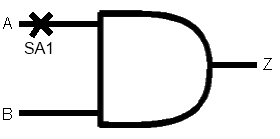
\includegraphics[scale=.7]{images/and-gate}
	\end{minipage}
	\begin{minipage}[r]{.45\textwidth}
		\begin{tabular}{|c|c|c|}
			\hline
			Inputs & Fault Free & Faulty \\
			(AB) & Output (Z) & Output (Z) \\ \hline
			0 0 & 0 & 0 \\ \hline
			0 1 & 0 & \multicolumn{1}{>{\columncolor[gray]{0.8}}c|}{1} \\ \hline
			1 0 & 0 & 0 \\ \hline
			1 1 & 1 & 1 \\ \hline
		\end{tabular}
	\end{minipage}
	\end{center}
	\caption{AND Gate with Input A Stuck-At `1'}
	\label{fig:andtruth}
\end{figure}
Since digital circuits will always produce the same outputs for a given set of inputs, any difference between the expected and actual output can be exploited to determine if a circuit is functioning correctly\cite{stroud}.  Each clock cycle an input vector is applied and the output is compared with the expected output.  If any output does not match the expected output then the chip is considered faulty and is discarded.  Unfortunately the storage required to hold each input and expected output vector can be significant for large or complex chips and while feasible for costly automatic test equipment, it is often impossible due to area considerations when using a BIST approach\cite{faultdiagnosis}.

When using BIST the input vectors are often generated by the TPG circuitry deterministically, algorithmically, or pseudo-randomly (among other methods)\cite{stroud}.  This keeps the size of the TPG to a minimum and removes the need for a large memory or other means of storing every input vector.  Likewise it is impractical to store every expected output pattern and compare it to the actual output each clock cycle.  To minimize storage requirements a signature is often used to compress the output of the circuit into a single vector.  Instead of comparing each output at the end of each clock cycle, the signature is generated during the test and compared to the expected signature at the end of a test\cite{stroud}\cite{faultdiagnosis}.  A signature can be generated in a number of different ways and may be as simple as a counter counting the number of 1's or 0's which occur in the output, 1's or 0's counting, or as complex as using a large Multiple Input Signature Register\nomenclature{MISR}{Multiple Input Signature Register}\cite{stroud}.  The most appropriate signature generation method is dependent on the requirements and output of the design and can significantly impact the effectiveness of a BIST approach.  If a method is used which does not produce a suitably unique signature then faulty circuits can escape detection\cite{stroud}\cite{faultdiagnosis}.  The use of an expected signature to compress the circuit output allows for a significant reduction in storage cost as in most cases only a single comparison needs to be performed to verify the circuit\cite{faultdiagnosis}.

Returning to the example in Figure \ref{fig:andtruth}, a simple BIST can be constructed to test the AND gate.  In Figure \ref{fig:andbist} a 2-bit counter is used as the TPG to generate all of the inputs patterns possible for a two input AND gate: ``00'', ``01'', ``10'', and ``11''.  Also in the figure the output of the AND gate is connected to the \textit{Enable} of an additional 2-bit counter to count each `1' and produce a signature.  The fault-free signature for this circuit is ``01'' since a normally operating AND gate should only produce a single logic `1' when both its inputs are logic `1'.  If any input is stuck-at `1' then it will produce at least one additional `1'; if any input is stuck-at `0' it will never produce a logic `1'.  These two conditions will produce invalid signatures.  During execution of the BIST sequence, the TPG counts from ``00'' to ``11'' and the 1's counter will increment for each `1' occurring at the output of the gate.  At the end of the sequence, if the value in the 1's counter is not ``01'' then the gate is faulty.  This example is greatly simplified and is missing required circuitry to start and stop the BIST as well as a method to isolate the inputs of the gate; however, it does demonstrate the general principal behind using BIST to test a digital circuit.

\begin{figure}
	\begin{center}
		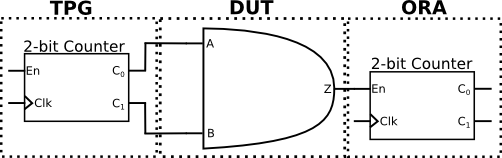
\includegraphics[scale=1]{images/and-bist}
	\end{center}
	\caption{Simple BIST for an AND Gate}
	\label{fig:andbist}
\end{figure}

\subsection{Analog Systems and Faults}
\label{sct:AnalogFaults}

Analog systems function differently than digital systems.  Unlike a digital system which only has two discrete values, analog systems are continuous waveforms with multiple levels and voltages\cite{syschip}.  In addition to the complexities of analog waveforms, analog components operate within a range of acceptable values\cite{syschip}.  This difference makes testing analog components for defects (defect-oriented testing) significantly more challenging and requires a more complex fault model.  In analog components faults are classified as either parametric (soft-faults) or catastrophic (hard-faults)\cite{analogfaults}.  Parametric faults are those which affect the performance of a specific component causing it to operate outside of its expected tolerance range, for example a resistor which has a lower than expected resistance.  In contrast catastrophic faults are those which cause a component to fail, such as resistor which is no longer conductive and appears as an open circuit\cite{analogfaults}.  The simulation of these different faults requires complicated and time consuming methods such as Monte Carlo analysis to determine different component values which allow fault-free circuit operation\cite{syschip}.  Compounding these issues is the fact that analog components
\begin{quote}
``function collectively to perform the overall functionality of a given circuit and, as a result cannot always be treated as a collection of individual components\cite{syschip}''
\end{quote}
and consequently are difficult to isolate for effective defect-oriented testing\cite{analogmixedtest}.  Furthermore any circuitry added into an analog circuit may potentially interfere and change the operating range or output of that circuit\cite{syschip}.  This potential interference requires that any analog testing circuitry be carefully simulated and verified to ensure it does not negatively affect the overall circuit performance.  An example of a defected-oriented approach, oscillation testing is a testing approach which reconfigures the analog CUT so that it oscillates; this oscillation frequency is then measured and compared to an expected frequency.  If the measured frequency falls outside the expected range, the circuit is considered faulty\cite{analogosc}.  This method has been shown to be effective for the detection of catastrophic faults and some parametric faults; however, it can require a significant amount of planning and design effort as it may significantly impact the analog circuitry\cite{analogosc}\cite{syschip}.

A simpler (and preferred\cite{syschip}) method for testing analog components is via functional testing. \cite{milor} defines functional tests as: 
\begin{quote}
``... those which measure a circuit's dynamic behavior ...\cite{milor}''
\end{quote}
Functional or specification testing is achieved by performing a set of tests to determine if a system is operating correctly as defined by its specifications.  This approach is used to test the entire analog system collectively instead of attempting to understand the implications of specific faulty components\cite{analogmixedtest}.  Specification testing may include the testing of important analog characteristics such as frequency response, linearity, and signal-to-noise ratio (SNR)\nomenclature{SNR}{Signal-to-Noise Ratio}\cite{syschip}; however, the characteristics which are important  to test will vary between designs.  To adequately test most analog components, multiple measurements of several different characteristics must be taken as a single characteristic is usually not sufficient to ensure fault-free operation\cite{analogmixedtest}.  This process may require extra development time as test procedures must be developed to test each characteristic and additional time is required to perform each test\cite{analogmixedtest}.

\subsection{Mixed Signal Testing}
\label{sct:MixedSignal}
In a mixed-signal environment both digital and analog systems coexist and interact.  Due to the previously discussed differences in testing analog and digital systems, the testing of the analog and digital sub-systems is generally developed separately and performed using using different test procedures and approaches\cite{analogmixedtest}.  Ideally a designer would like to limit any duplicate work and take advantage of a BIST approach which can be used to test both the analog and digital sub-systems.

\cite{stroud} defines a BIST approach to testing mixed-signal systems shown in Figure \ref{fig:mixedbist1}.  This BIST uses a digital BIST approach to functionally test the analog sub-system by measuring certain analog characteristics which can be used ensure that the circuit is operating within its specifications.  This architecture is largely digital and thus can be integrated into the digital circuitry already in the system with minimal analog overhead.  This prevents excessive interference with the analog circuitry, excluding analog multiplexers which facilitate the sending and retrieving of test values to and from the analog sub-system\cite{stroud}.  To test the analog circuitry, the BIST uses the existing digital to analog converter (DAC) to convert digitally generated test patterns from the TPG to analog signals and the existing analog to digital converter (ADC) to convert the analog response back into the digital domain for analysis by the ORA\cite{stroud}.
\begin{figure}
	\begin{center}
		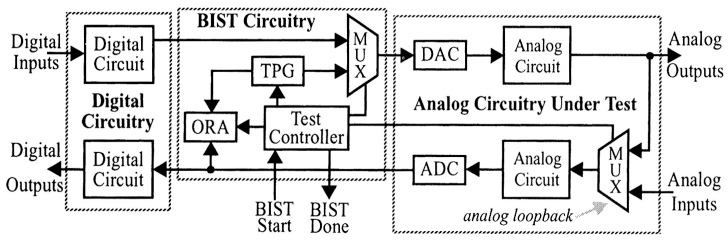
\includegraphics[scale=1]{images/mixed-bist-architecture}
	\end{center}
	\caption{BIST Approach for Mixed-Signal Systems\cite{stroud}}
	\label{fig:mixedbist1}
\end{figure}

Figure \ref{fig:mixedbist1} shows a basic version of this mixed-signal BIST approach using two multiplexers.  In this case one multiplexer is placed before the DAC to select between the BIST patterns and the system circuitry and a second multiplexer is positioned at the input of the analog system to select between the system level inputs and the analog outputs.  These two multiplexers form a loop allowing the generated TPG pattern to be converted into an analog signal and propagate through any analog circuitry before being routed back through the analog inputs to the DAC for analysis by the ORA.  While this implementation does allow testing of all analog components, it does not allow a high level of diagnostic resolution\cite{syschip}.  To obtain a higher diagnostic resolution, additional analog multiplexers can be added to further partition the system. Figure \ref{fig:mixedbist_paths} shows an example of an implementation with three separate multiplexed or loopback paths to facilitate a higher level of diagnostic resolution.  In Figure \ref{fig:mixedbist_paths} the shortest loop, the short dashed path, is a digital only path (digital loopback path) which can be used to test that the digital BIST is fault-free.  The next loopback path, the dashed path, connects the output of the DAC to the ADC bypassing any of the analog circuitry (from here on referred to as the bypass path).  This allows the verification of the ADC and DAC separately from the analog circuit.  The final path is the analog test path, the dotted path, and is similar to the path in Figure \ref{fig:mixedbist1} in that it is responsible for testing the analog circuitry.  There is no limit to the number of multiplexers that can be added to the system other than the increase in area overhead\cite{syschip}.  Additional analog multiplexers could be added to the example in Figure \ref{fig:mixedbist_paths} to further partition the analog circuitry and resolve faulty behavior to a specific portion of the analog DUT.
\begin{figure}
	\begin{center}
		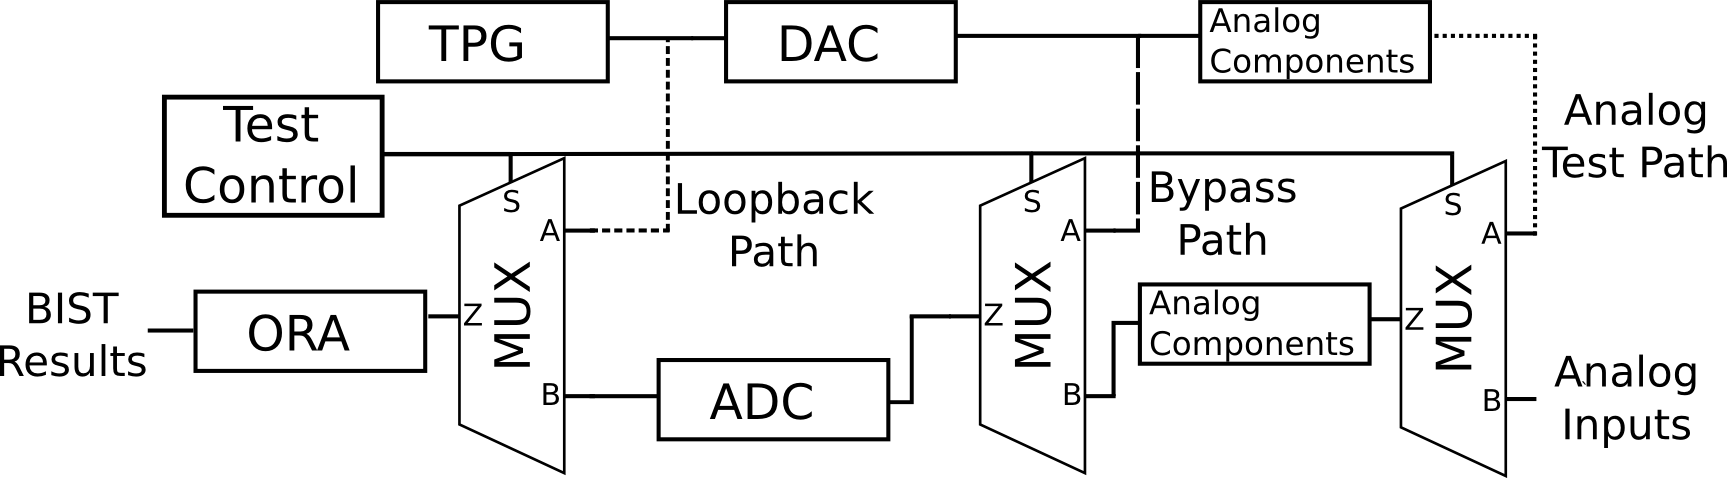
\includegraphics[scale=1]{images/mixedbist-paths}
	\end{center}
	\caption{Mixed-Signal BIST with Multiple Loopback Paths}
	\label{fig:mixedbist_paths}
\end{figure}

In Figure \ref{fig:mixedbist_paths} the digital loopback path is of particular importance.  \cite{stroud-analog} has shown that a digital loopback path is highly advantageous when testing the digital portion of the BIST circuitry.  In a digital only environment the BIST produces exactly one output for a given set of inputs; however, without the digital loopback path the TPG outputs are not directly observable.  To observe the outputs of the TPG requires conversion via the DAC and reconversion via the ADC.  This will cause variations in the expected results due to the inherent variations which occur in analog signals and circuits.   To account for these variations, a range of acceptable values must be considered instead of an exact signature\cite{stroud-analog}.  

Figure \ref{fig:analog-faultcvg}
\begin{figure}
	\begin{center}
		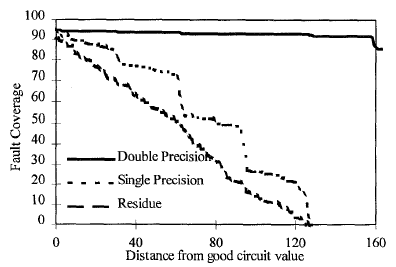
\includegraphics[scale=.7]{images/analog-fault-coverage}
	\end{center}
	\caption{Fault Coverage v. Acceptable Value Range\cite{stroud-analog}}
	\label{fig:analog-faultcvg}
\end{figure}
shows a comparison of the maximum achievable digital fault coverage versus the allowed distance away from the expected good signature for different ORA designs.  In the figure, three different 8-bit ORA accumulator designs are considered  (ORA design is discussed in more detail in the next chapter).   Figure \ref{fig:analog-faultcvg} shows that regardless of design a (in some cases significant) reduction in the maximum achievable fault coverage is to be expected when a range of good values is considered instead of an exact signature.  Thus the only way to achieve the maximum fault coverage is to not use a range of acceptable values and perform a digital only test.  This requires the digital loopback path\cite{stroud-analog}.  Performing a digital only test separates the digital and analog systems when testing.  This allows for the usage of tools and techniques which target digital components separately from those used to generate the analog functional tests on the analog sub-system\cite{stroud-analog}.  When the three loopback paths shown in Figure \ref{fig:mixedbist_paths} are present, the test procedure should be performed first over the digital loopback path to verify the digital BIST, then using the bypass path to verify that the ADC and DAC path are functioning correctly, and finally over the entire circuit to verify the analog DUT\cite{syschip}\cite{stroud-analog}.

Though this technique still requires the separate testing of the analog and digital circuitry, it is an improvement over the previously discussed method since the same BIST circuitry can be used to test both the digital and analog circuitry\cite{stroud}.  This limits the amount of work that must be duplicated to the determination of which tests must be run and the expected values or range of values that must be considered.  Furthermore the basic procedure for testing the analog and digital circuits is the same (the only differences being which loopback path is selected and the actual test being performed) which will limit the differences between test sessions.

\section{Summary}
In this chapter a high-level look at both digital and analog systems has been given as well as the challenges of testing these systems for faults.  The concept of BIST has been presented along with its advantages and a simple BIST architecture.  In addition the challenges of testing mixed-signal systems has been discussed and a basic mixed-signal BIST model has been given along with an overview of the challenges of testing the BIST without a digital loopback path.  In the next chapter a more detailed explanation of fault simulation and of the specific mixed-signal BIST approach studied in this thesis is given.  This approach builds upon the simple architecture discussed in the previous section and addresses the challenges discussed in Section \ref{sct:AnalogFaults}.  Building upon this explanation, Chapter III explores the preparation necessary for simulating the mixed-signal BIST including necessary conversions and verification.  Chapter IV explores the main topic of this thesis: testing the actual mixed-signal testing circuitry to determine the level of fault coverage achievable.  Methods for improving the BIST and the maximum achievable fault coverage are explored before a summary and conclusions are given in Chapter V.

\chapter{Background}
Before discussing the fault simulations performed in this thesis, it is important to have a more thorough understanding of fault simulation techniques.  In this chapter, an overview of several fault simulation techniques will be given as well as an overview of the bridging fault model which models faults between nets.  Following this discussion a more detailed outline of the simulation and design process will be given.  Next the fault simulator AUSIM\nomenclature{AUSIM}{Auburn University SIMulator} is detailed which is used to evaluate the fault coverage of the mixed-signal BIST approach studied in the rest of this thesis.  This chapter concludes with a detailed discussion of the architecture of the mixed-signal BIST and its capabilities.

\section{Fault Simulations}
\label{sct:faultsim}
% An introduction to fault simulation is probably appropriate
Knowledge of the basic concepts of simulation is important to understanding how fault simulations are performed.  The simulation process begins with a netlist.  The netlist represents the circuit design to be simulated and defines the structure of the circuit at the gate level.  This includes both the gates used by the circuit as well as the interconnections between those gates\cite{advancedverilog}.  The generation of a netlist is discussed in more detail in Section \ref{sct:designprocess}.  According to Section \ref{sct:basictesting}, the next step is to generate a set of test vectors to be used to stimulate the circuit during testing.  Test vectors may be generated automatically using Automatic Test Pattern Generation (ATPG)\nomenclature{ATPG}{Automatic Test Pattern Generator}\cite{advancedverilog} or manually by the designer.  When performing fault simulations, these vectors should ideally exercise as much of the internal circuitry of the design as possible so that high fault coverage can be achieved (fault coverage is discussed towards the end of this section); consequently, test vectors generated using  ATPG can be advantageous as they typically guarantee a very high fault coverage\cite{advancedverilog}.  If vectors are created manually by the designer then it may be necessary to perform a logic simulation of the circuit to ensure the vectors are valid and to obtain the fault-free output of the circuit (when using ATPG the fault-free output is generally recorded along with the test vector set).  With both the test vector set generated and fault-free output of the circuit known, fault simulations can begin.  

Fault simulation starts with the selection of a fault model which characterizes the fault behavior to be simulated.  There are several different fault models used for digital circuits, but the focus of this thesis will be the gate-level stuck-at fault model which was introduced in Section \ref{sct:digitalsystems}.  The stuck-at fault model has a low computation cost and accurately represents the behavior of faults seen at the gate-level of digital circuits\cite{stroud}.  Other models exist which characterize different fault behavior and have their own set of advantages and disadvantages.  The bridging fault model, which will be introduced in Section \ref{sct:bridgingfaults}, focuses on faults which occur between nets as opposed to those that occur at gate inputs and outputs and is used to accurately simulate faults that occur in circuit routing\cite{stroud-bridging}.  The transistor fault model targets faults which occur at the transistor level.  This level of detail makes it more computationally expensive to simulate compared to the gate-level model; however, this model more accurately represents the behavior of faults which occur during the manufacturing process\cite{defectforcmos} and may detect faults which are not detectable using the stuck-at fault  model.  Regardless of its accuracy, it is more common to use the gate-level stuck-at model for digital fault simulations since it is less computationally expensive and is acceptably accurate at modeling the behavior of common defects in digital systems\cite{defectforcmos}.  

Once a fault model is chosen each fault must be simulated and the output of the circuit recorded.  The output of the faulty circuit is compared to the fault-free output and if any discrepancy is found then the fault is recorded as detected.  Similarly if the output of the circuit is always the same as the fault-free circuit then the fault is not detected\cite{defectforcmos}.  In some cases a fault may be considered potentially detected; this special case is caused by an unknown logic value occurring in the circuit and is an artifact of simulation.  An unknown logic value will occur if a circuit element is not initialized properly\cite{stroud}.  In physical hardware the value must be either logic `0' or logic `1'; however, in simulation it is unknown which logic value it will initialize to which causes the detection of the fault to be uncertain in simulation\cite{stroud}.  The percentage of faults detected is said to be the fault coverage of the test vector set\cite{defectforcmos}\cite{stroud}.  Fault coverage is typically calculated using Equation \ref{equ:faultcvg} where $D$ is the number of detected faults, $P$ is the number of potentially detected faults, $Y$ is the probability of potentially detected faults being detected, $X$ is the number of undetectable faults and $T$ is the total number of faults simulated\cite{stroud}.  
\begin{equation}
F_C = \frac{(D + (Y \times P))}{(T - X)}
\label{equ:faultcvg}
\end{equation}
Undetectable faults are faults which are impossible to detect by any test vector.  These faults are often caused by design issues such as re-convergent fan-out and redundant logic\cite{stroud} and since they cannot be detected are typically not considered when calculating fault coverage.  In the equation $Y$ is typically $.5$ denoting that there is a 50\% chance of a potentially detected fault being detected.  This represents the chance of an uninitialized logic value initializing to the logic value required for detection when testing is performed in physical hardware.  This coefficient may be changed to represent a higher or lower chance of detecting potentially detectable faults\cite{stroud}.

For a large number of faults or large number of test vectors the simulation process can take a large amount of time to complete. In the worst case the time required to complete a fault simulation is shown in Equation \ref{equ:fsimtime}, where $T_{vec}$ is the time required to simulate a single vector, $N_{vec}$ is the number of test vectors to be simulated, and $N_{flts}$ is the number of faults to be simulated.  
\begin{equation}
Time = T_{vec} \times N_{vec} \times N_{flts}
\label{equ:fsimtime}
\end{equation}
There are a couple of methods which can decrease the amount of time taken to simulate a list of faults.  One common method is fault dropping.  When using fault dropping a fault is only simulated until a discrepancy between the output of the circuit and the fault-free output is found.  At that point the fault is recorded as detected, simulation of the fault is halted, and a new fault is simulated\cite{stroud}.  The time required to perform fault simulation when using fault dropping is shown in Equation \ref{equ:fdroptime} where $N_{flts}$ is the number of faults to be simulated, $T_{vec}$ is the time required to simulated a single vector, and $N_{vec_i}$ is the number of vectors simulated for the $i^{th}$ fault.
\begin{equation}
Time =  \sum_{i=0}^{N_{flts}} T_{vec} \times N_{vec_i}
\label{equ:fdroptime}
\end{equation}
In the case where the $i^{th}$ simulated fault is detected early in the simulation, $N_{vec_i}$ will be small shortening the simulation time for the fault; in contrast, if the $i^{th}$ fault is detected toward the end of the simulation or not detected at all then $N_{vec_i}$ will be approximately $N_{vec}$ causing little to no savings in simulation time for the fault\cite{stroud}.  

Further speed up can be obtained by performing parallel fault simulation.  Equations \ref{equ:fsimtime} and \ref{equ:fdroptime} show the time required to perform serial fault simulations where a single fault is simulated at a time.  To decrease the time required for simulation, it is beneficial to simulate multiple faults concurrently\footnote{This does not mean perform the simulation of multiple faults in the same circuit simultaneously; but instead, it means perform multiple simulations in parallel each with a single fault\cite{parallelflts}}. This is a common approach to decreasing simulation time and at least in the case of gate-level stuck-at fault simulation, does not require any additional considerations by the user\cite{parallelflts}.  Commonly 32 faults\footnote{An integer is 32-bits on a 32-bit machine; consequently, simulating 32 faults allows for the use of the integer data type in the simulator and makes parallel fault simulation easier to implement\cite{parallelflts}} are simulated in parallel though different simulators may have options to simulate more or less faults\cite{parallelflts}.  Equation \ref{equ:psimtime} defines the worst case time required to perform parallel fault simulation and Equation \ref{equ:psimdroptime} defines the time required to perform parallel fault simulation with fault dropping assuming 32 faults are simulated in parallel (in this case $N_{vec}$ is the number of vectors required to detect all faults in a parallel group). 
\begin{equation}
Time = T_{vec} \times N_{vec} \times \frac{N_{flts}}{32}
\label{equ:psimtime}
\end{equation}
\begin{equation}
Time =  \sum_{i=0}^{[\frac{N_{flts}}{32}]} T_{vec} \times N_{vec_i}
\label{equ:psimdroptime}
\end{equation}
Using both fault dropping and parallel fault simulation can greatly decrease the required simulation time for a large circuit.  Due to this benefit both of these methods are used in the fault simulations performed in this thesis.  The next section discusses further optimizations which can be performed to reduce the number of faults simulated and consequently the time required to perform simulation.

\subsection{Collapsed vs Uncollapsed Faults}
% This should discuss collapsed vs uncollapsed as it relates to the stuck-at fault model
% An image showing some faults and the collapsed version (similar to Dr. Strouds image from BIST would be good)
% Can greatly improves simulation time, disadvantages? FC related I guess?
% give an example of the difference: use the BIST... why not
When performing fault simulations certain optimizations can be made to improve the efficiency of the simulation.  One such optimization is fault collapsing.  With the gate-level single stuck-at fault model, each gate input and output can be stuck-at logic `0' or logic `1'.  For elementary logic gates this leads to many faults which produce identical faulty behavior; these faults can be said to be equivalent\cite{defectforcmos}.  During simulation these equivalent faults can be collapsed, requiring only a single fault out of the group of equivalent faults to be simulated\cite{defectforcmos}.  Depending on the circuit this can substantially reduce the number of faults to be simulated while still accurately representing the faults which can occur in the circuit\cite{defectforcmos}.  Figure \ref{fig:faultcollapse} shows an example of fault collapsing.  The NOR gate in the figure has six uncollapsed faults; however, when either input is stuck-at `1' it is equivalent to the output being stuck-at `0' and vice versa (since a logic `1' is the controlling input for a NOR gate) which results in four collapsed faults.  These equivalent faults are shown in bold in the figure.
\begin{figure}
	\begin{center}
		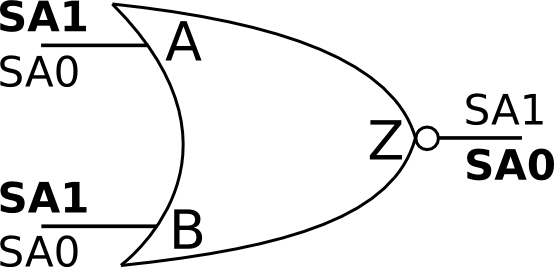
\includegraphics[scale=1]{images/nor-faultcollapse}
	\end{center}
  \caption{NOR Gate with Six Uncollapsed and Four Collapsed Faults}
  \label{fig:faultcollapse}
\end{figure}
\cite{stroud} states that the number of collapsed faults for any elementary logic gate with greater than one input is $K+2$ where $K$ is the number of inputs to the gate.  This is certainly apparent with the NOR gate in Figure \ref{fig:faultcollapse}, where $K+2=4$.  Additionally when the output of a gate is connected to exactly one input of another gate, a fault occurring at the output of the source gate is indistinguishable from the same fault occurring at the input of the connected gate\cite{stroud}.  These faults can be structurally collapsed together which leads to a large chain of faults being collapsed such as the example in Figure \ref{fig:collapsechain}\cite{stroud}.  In the figure groups of equivalent faults are shown with a line drawn between them.  Unfortunately due to the limitation of the single stuck-at fault model, which does not allow multiple faults to appear in the circuit simultaneously (as opposed to a multiple fault model which allows this), the fan-out stem in Figure \ref{fig:collapsechain} cannot be collapsed\cite{defectforcmos}.  Since the output of the inverter fans-out to the input of two different gates, collapsing these faults would make a fault appear to be on both the input of the AND gate and the OR gate simultaneously which violates the single stuck-at fault model and is not allowed\cite{defectforcmos}.  Counting the faults in the figure, there are a total of 22 uncollapsed faults and a total of 12 collapsed faults, a significant reduction.
\begin{figure}
	\begin{center}
		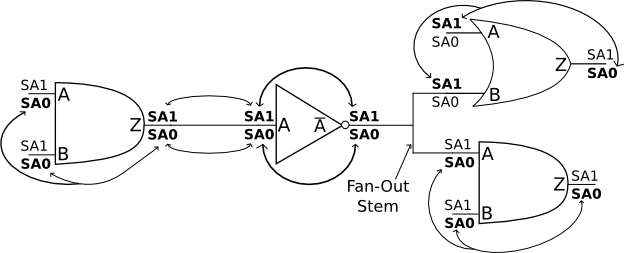
\includegraphics[scale=1]{images/faultchain-collapse}
	\end{center}
  \caption{Structural Fault Collapsing Performed on a Group of Logic Gates}
  \label{fig:collapsechain}
\end{figure}

In the single stuck-at fault model the number of uncollapsed faults in a circuit are $2 \times G_i_o$ where $G_i_o$ is the number of gate inputs and outputs in the circuit\cite{stroud}.  In contrast the number of collapsed faults can be determined by Equation \ref{equ:collapse-eq} where $P_o$ is the number of primary outputs, $F_o$ is the number of fan-out stems, $G_i$ is the number of gate inputs, and $N_i$ is the number of inverters in the circuit\cite{stroud}.
\begin{equation}
F = 2(P_o + F_o) + G_i - N_i
\label{equ:collapse-eq}
\end{equation}
As an example, the BIST model evaluated in this thesis has a total of 83386 uncollapsed faults.  It has 30 primary outputs, 4436 fan out stems, 27861 gate inputs, and 2740 inverters.  By using Equation \ref{equ:collapse-eq} the number of collapsed faults in the BIST circuitry is 34053.  This results in a 59\% reduction in the number of faults to be simulated.  

\cite{stroud} discusses the advantages and disadvantages of using the collapsed or uncollapsed fault set for simulation purposes.  According to \cite{stroud} it is obvious that the simulation time can be greatly reduced by using the collapsed fault list.  This is very advantageous as more simulations can be performed in the same amount of time.  However, \cite{stroud} does say that the uncollapsed fault list more accurately represents the possible defects which occur during manufacturing.  Due to this difference, the fault coverage obtained with the collapsed fault list may be different than the coverage according to the uncollapsed fault list by a few percent\cite{stroud}.  Through the accuracy of the uncollapsed fault list is preferable, the collapsed fault list is more often used due to its decreased simulation time\cite{stroud}.


\subsection{The Bridging Fault Model}
\label{sct:bridgingfaults}
% Discuss multiple models
% Discuss in detailed dominant model
% Discuss collapsed vs uncollapsed
% Can be difficult to simulate due to large number of faults sites (N^2-N)/2
Though the focus of this thesis is gate-level stuck-at fault simulations, additional models may be of interest for future work; specifically bridging fault simulations are commonly performed to assess the fault coverage of faults which occur between nets.  There are a number of different fault models which describe the behavior of bridging faults, faults where two nets are shorted together due to a manufacturing defect, including the Wired OR/AND, Dominant, and Dominant OR/AND fault model\cite{stroud-bridging}.  In this section we will focus on the dominant bridging fault model as it is the most commonly used\cite{stroud}.  For many years it was a commonly held belief that a high stuck-at fault coverage provided a high bridging fault coverage; however, more recent work has shown that this is not always the case and that it is important to perform these simulations separately to ensure that an acceptably high bridging fault coverage is achieved\cite{stroud-bridging-physical}.  Unfortunately bridging fault simulation can be significantly more time consuming than stuck-at fault coverage due to the large number of fault sites that must be considered.
\begin{equation}
F_B = (N^2-N)/2
\label{equ:bridging-fault-sites}
\end{equation}
Equation \ref{equ:bridging-fault-sites} shows the calculation to determine the number of possible bridging fault sites in a circuit, where $N$ is the number of nets in the circuit\cite{stroud}.  Like the previous section, the BIST model can be used to give a sense of scale.  The BIST studied in this thesis has 15221 nets, by applying Equation \ref{equ:bridging-fault-sites} the number of bridging fault sites is 115,831,810.  Depending on the bridging fault model up to four faults (when using the Dominant AND/OR model\cite{stroud-bridging}) are possible at each fault site, so this means that the worst case number of faults to be simulated is almost 500 million!  Similar to the gate-level model, bridging faults can also be structurally collapsed which can substantially lower the number of faults to be simulated (using the same circuit the number of collapsed faults was approximately 30K when using the more common dominant model).

As discussed in the previous paragraph, there are different models to define the types of bridging faults which can occur.  Since it is the most common, the dominant bridging fault model will be discussed.  According to the dominant bridging fault model, two different faults can occur at a bridging fault site: net A can dominate net B or net B can dominate net A.  Whichever net is dominated will be affected by the other net's current logic value; this occurs due to the dominate net having a stronger drive transistor\cite{stroud-bridging}.  Figure \ref{fig:bridgingfault} shows an example of a dominant bridging fault where net A dominates net B, along with a truth table containing the fault-free and faulty behavior of the circuit.  
\begin{figure}
  \begin{center}
    \begin{minipage}[l]{.55\textwidth}
      \begin{center}
        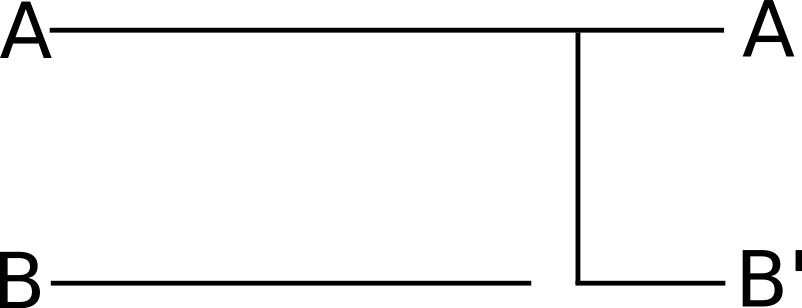
\includegraphics[scale=.8]{images/bridgingfault}	
      \end{center}
    \end{minipage}
    \begin{minipage}[r]{.35\textwidth}
      \begin{center}
        \begin{tabular}{|l|l|l|}
          \hline
          Net A & Net B & Faulty' \\ 
          & & Net B' \\ \hline
          0 & 0 & 0 \\ \hline
          0 & 1 & 0 \\ \hline
          1 & 0 & 1 \\ \hline
          1 & 1 & 1 \\ \hline
        \end{tabular}
      \end{center}
    \end{minipage}
  \end{center}
  \begin{center}
		\begin{minipage}[l]{.55\textwidth}
      \begin{center}
        (A)
      \end{center}
		\end{minipage}
		\begin{minipage}[r]{.35\textwidth}
      \begin{center}
        (B)
      \end{center}
		\end{minipage}
	\end{center}
  \caption{Bridging Fault where Net A Dominates Net B}
  \label{fig:bridgingfault}
\end{figure}
When net B has the same logic value as net A its output is unaffected; however, when the logic value of net B is different than that of net A, net B's logic value will be changed to that of net A.  The first two columns of the truth table in Figure \ref{fig:bridgingfault} represent the fault-free behavior of net A and net B and the remaining column B' represents the faulty output of net B when net A dominates it.  In the second row when net A is a `0' and net B should be a `1', B' is instead a `0' since it is dominated by net A.  Likewise in the third row when net A is a `1', net B should be a `0' but instead is a `1' due to the influence from net A.

Bridging faults are important to address during the design of a circuit.  Unfortunately they can be computationally expensive and can be difficult to test and observe\cite{stroud-bridging}.  Bridging faults were not simulated in this thesis though it is a target of future work.

\subsection{Design Process}
\label{sct:designprocess}
% Discuss behavioral -> place and route -> post-layout
% Advantages of simulating post-layout
% Transition into discussion on converting post-layout netlist (A tool was written for this purpose and is discussed in Chapter 3)
The design of a digital circuit typically starts with a behavioral description of a circuit.  This is generally done in a high-level design language such as Verilog or VHSIC Hardware Design Language (VHDL)\nomenclature{VHSIC Hardware Design Language}{VHDL} and usually will not include any implementation details of the circuit\cite{advancedverilog}.  This code is then fed into a synthesis computer-aided design (CAD)\nomenclature{CAD}{Computer-Aided Design} tool which will interpret the behavioral description of the design, combine it with parameters such as the implementation technology, timing information, and/or area constraints, and ultimately produce a gate-level netlist of the design\cite{advancedverilog}.  Following this step a place-and-route tool takes each gate and its interconnections and decides where on the silicon chip (or in a field-programmable gate array (FPGA)\nomenclature{FPGA}{Field-Programmable Gate Array} or other programmable device) to place the gate so that any timing and area constraints can be achieved.  Once completed the design is said to be ``post-layout'' indicating it is ready for fabrication\cite{advancedverilog}.

Logic simulation is important during each step of this design process, so that the circuit behavior can be verified before fabrication\cite{advancedverilog}.  During the behavioral modeling phase, design verification is performed to ensure the description of the circuit is correct and that no design errors have been made.  Simulation is also performed after synthesis has taken place to verify that the circuit's behavior is still correct after it has been implemented at the gate-level and to investigate any potential timing problems with the circuit\cite{advancedverilog}.  Following post-synthesis simulation, post-layout simulation is also performed.  Post-layout represents the final version of the circuit to be fabricated.  Simulation can be performed using the circuit's final timing information and can incorporate many different performance characteristics.  Post-layout is the final opportunity to verify a circuit is functioning correctly before fabrication\cite{advancedverilog}.

In contrast to logic simulation, fault simulation is not typically performed at any of the high-level steps in the design process\cite{stroud}.  Ideally the post-layout netlist should be used for all fault simulations, since the layout can have a significant impact on the faults in a circuit\cite{defectforcmos}.  This is especially true of bridging fault simulations as routing is not finalized until the layout stage and thus cannot be accurately performed earlier in the design process\cite{defectforcmos}; however, other fault models may be simulated earlier in the design verification process\cite{stroud}.  In this thesis all fault simulations of the BIST are performed using the post-layout design.  As discussed in the next chapter, this does present a challenge since the post-layout design produced by the CAD tools is a Verilog netlist which is not a format used by the fault simulator.  As such a tool was written to convert a Verilog netlist to the ASL netlist format recognized by our simulator AUSIM (ASL and the fault simulator AUSIM will be discussed in Section \ref{sct:ausim}).

\section{AUSIM Fault Simulator}
\label{sct:ausim}
% Some discussion on the general use of the simulation
% Capabilities
For the fault simulations performed in this thesis the Auburn University SIMulator or AUSIM is used.  Developed by Dr. Charles Stroud\cite{ausim}\cite{asl}, AUSIM can perform both logic and fault simulations.  In addition it supports multiple fault models including the gate-level stuck-at and multiple bridging fault models\cite{ausim}.  It supports all of the previously discussed methods of improving simulation time including fault collapsing and parallel fault simulation of both bridging and stuck-at faults\cite{ausim}.  A detailed description of the operation and usage of AUSIM will not be given in this thesis; however, more information can be found in \cite{ausim}\cite{asl}; instead, the focus of this section is an overview of the Auburn Simulation Language or ASL\nomenclature{ASL}{Auburn Simulation Language} which is the netlist format used by AUSIM.

\subsection{ASL Netlist Format}
\label{sct:ASL}
% Format used by AUSIM for simulations
% Discussion of the specifics
Before a circuit can be simulated by AUSIM it must be in a format that AUSIM can understand.  The Auburn Simulation Language (ASL)\nomenclature{ASL}{Auburn Simulation Language} is the circuit description used by AUSIM\cite{asl}.  ASL is used to provide a textual representation of a circuit at the gate-level to the simulator.  This gate-level net-list is used to describe each connection and gate used in a circuit design and allows the simulator to build a representation of the circuit under test.  ASL begins with a top-level circuit declaration.  This declaration defines the name of the circuit and uses the \textit{in} and \textit{out} keywords to define the inputs and outputs to the circuit\cite{asl}.  An example circuit is given in Figure \ref{fig:half_adder}.  Figure \ref{fig:half_adder} A is a half-adder which takes in two inputs and outputs a sum (S) and carry bit (C), the corresponding ASL description is given in Figure \ref{fig:half_adder} B.
\begin{figure}
	\begin{center}
		\begin{minipage}[l]{.45\textwidth}
			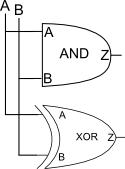
\includegraphics[scale=1]{images/half-adder}	
		\end{minipage}
		\begin{minipage}[r]{.45\textwidth}
			\begin{center}
				Half-Adder Circuit
			\end{center}
			\begin{enumerate}
				\setlength{\itemsep}{0cm}
				\item \# Half-Adder ;
				\item ckt: HF in: A B out: S C ;
				\item xor: X1 in: A B out: S ;
				\item and: A1 in: A B out: C ;
			\end{enumerate}
		\end{minipage}
	\end{center}
	\begin{center}
		\begin{minipage}[l]{.45\textwidth}
			(A)
		\end{minipage}
		\begin{minipage}[r]{.45\textwidth}
			(B)
		\end{minipage}
	\end{center}
	\caption{A Half-Adder Circuit}
	\label{fig:half_adder}
\end{figure}
As can be seen from the figure the circuit declaration is started by the \textit{ckt} keyword\cite{asl}.  Each keyword in ASL is followed by a `:' character\cite{asl}.  Following the \textit{ckt} keyword is the name of the circuit in this case ``HF''.  Following that, the primary inputs and outputs are declared using the \textit{in} and \textit{out} keywords.  Each statement in ASL is terminated using a `;' character\cite{asl}.  After the circuit statement the gate-level description of the circuit is given.  The format of each gate is similar to the format of the circuit statement:
\begin{quote}
	\textbf{GATE}: Name \textbf{IN}: In1 In2... InN \textbf{OUT}: Out1 Out2... OutN ;\cite{asl}
\end{quote}
All gate declarations in ASL follow this simple syntax.  All of the elementary logic gates (AND, OR, XOR, etc..) as well as the data flip-flop (DFF)\nomenclature{DFF}{Data Flip-Flop} and two input multiplexer are built-in to AUSIM and available to all circuits\cite{asl}.  Table \ref{tbl:ASLGates} shows each built-in gate and its inputs and outputs.
\begin{table}[bht]
\caption{Built-In AUSIM Gates\cite{asl}}
\begin{center}
\begin{tabular}{|l|l|}
\hline
\multicolumn{2}{|c|}{AUSIM Keywords} \\ \hline
Gate & Example \\ \hline
AND & AND: a1 in: i1.. iN out: Z ; \\ \hline
OR & OR: o1 in: i1.. iN out: Z ; \\ \hline
NAND & NAND: na1 in: i1.. iN out: Z ; \\ \hline
NOR & NOR: no1 in: i1.. iN out: Z ; \\ \hline
NOT & NOT: n1 in: A out: Z ; \\ \hline
XOR & XOR: x1: in: i1... iN out: Z ; \\ \hline
MUX2 & MUX2: m1 in: i1 i2 s1 out: Z ; \\ \hline
DFF & DFF: d1 in: CLK D out: Q Qn ; \\ \hline
\end{tabular}
\end{center}
\label{tbl:ASLGates}
\end{table}

It is important to understand that custom gates can be implemented hierarchically and used in a similar syntax.  To do this one must use the \textit{subckt} command.  While an ASL file can only have a single circuit declaration, it can have any number of sub-circuit declarations\cite{asl}.  Each sub-circuit has its own set of top-level inputs and outputs and its own gate-level net-list.  Once defined the name of the sub-circuit can be used as a gate and be instantiated elsewhere in the circuit description.  These sub-circuit definitions can be used to define the behavior of more complex CMOS standard cell gates such as the OAI222 etc.  For the BIST discussed in this thesis, an entire library of sub-circuits was created to support simulation.  This library defines many of the complex CMOS logic gates and several technology specific standard cells used by the BIST circuitry.  This library is discussed in more detail in Chapter 3.

\section{BIST Architecture}
% Introduce the bist, its SSA BIST based on a DDS
% some other introductory characteristics
The BIST architecture analyzed in this thesis is a mixed-signal BIST approach which uses Selective Spectrum Analysis (SSA)\nomenclature{SSA}{Selective Spectrum Analysis} to functionally test analog circuitry\cite{jie-journal}.  SSA has many advantages when used to measure frequencies in an analog spectrum.  First it benefits from being a largely digital approach and integrates well into a BIST environment.  In addition, due to SSA measuring only a single frequency point at a time, the hardware overhead is much lower when compared to alternative approaches such as FFT\cite{stroud-phase}. However, since only a single frequency is measured at one time, test time can become long when a large number of frequencies are of interest.  Likewise SSA can prove very advantageous when only a few frequencies are of interest in the analog spectrum\cite{jie-journal}.  Furthermore, \cite{jie} discusses a number of optimizations detail (some of which will be discussed in Section \ref{sct:bist-ora}) which when used can greatly reduce the time required to perform a measurement.

\begin{figure}
	\begin{center}
		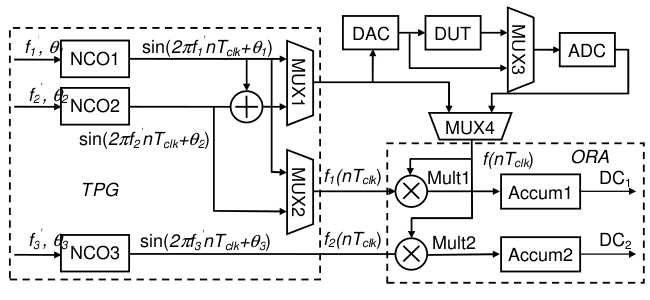
\includegraphics[scale=.5]{images/bist-ssa-architecture}
	\end{center}
	\caption{General BIST Architecture\cite{testtime}}
	\label{fig:bist-ssa}
\end{figure}
A block diagram of the basic architecture of the SSA BIST approach can be seen in Figure \ref{fig:bist-ssa}.  This BIST architecture is capable of measuring a number of different analog characteristics including the frequency response and linearity (also known as third-order interception point or IP3\nomenclature{IP3}{Third Order Interception Point}) of a DUT\cite{basessa}.  In addition by sweeping through a frequency spectrum both Signal-to-Noise Ratio (SNR) and Noise Figure\cite{noisefigure} and be measured.  The architecture in Figure \ref{fig:bist-ssa} consists of a Direct Digital Synthesis (DDS)\nomenclature{DDS}{Direct Digital Synthesis} based TPG, Multiplier-Accumulator (MAC)\nomenclature{MAC}{Multiplier Accumulator} based ORA, and test controller (not shown).  Also not shown in the figure is an on-chip calculation circuit which will be discussed in Section \ref{sct:onchip}.  The following sections will discuss each of the major BIST components and discuss how each test is performed and calculated so that the reader can develop an understanding of the capabilities and uses of this BIST architecture as it pertains to this thesis.

\subsection{DDS Based TPG}
% Discuss DDS based frequency generation
% Discuss frequency words and how they relate to the clock speed and frequency generation
DDS is a popular technique for generating analog frequencies on chip.  Compared to other techniques of frequency generation it offers the ability to produce very precisely controlled frequencies which can be rapidly manipulated and changed using digital inputs\cite{qi}.  In addition with adequate design considerations, DDS designs can have extremely fine frequency and phase resolution.  The BIST TPG is DDS based consisting of three numerically controlled oscillators (NCOs)\nomenclature{NCO}{Numerically Controlled Oscillator} which utilize the existing DAC in the mixed-signal system to generate the analog waveforms for testing\cite{testtime}.  Each NCO utilizes a phase accumulator and sine/cosine lookup table (LUT)\nomenclature{LUT}{Lookup Table} to produce a frequency based on a supplied frequency word $f_w$. The supplied frequency word is accumulated each clock cycle by the phase accumulator.  The value of the phase accumulator is truncated and used as a lookup address to find the appropriate sine or cosine value in the LUT.  The value retrieved from the LUT is then converted by the DAC into an analog signal.  The basic steps of this process are shown in Figure \ref{fig:dds}.  
\begin{figure}
  \begin{center}
		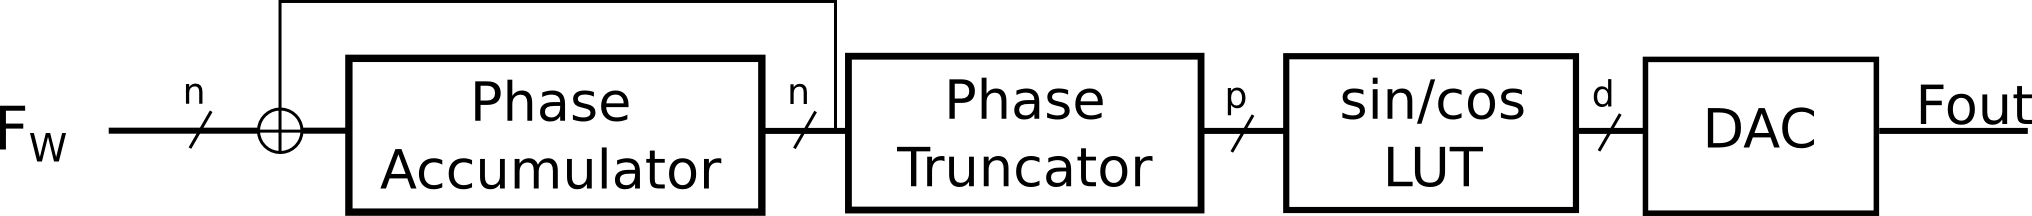
\includegraphics[scale=.8]{images/dds-steps}
  \end{center}
  \caption{Block Diagram of DDS}
  \label{fig:dds}
\end{figure}
The resulting frequency generated by the NCO is determined by Equation \ref{eq:frequencyword}, where $f_{gen}$ is the generated sine wave frequency, $f_w$ is the supplied frequency word, $f_{clk}$ is the system clock frequency, and $n$ is the number of bits in the frequency word.  The maximum frequency resolution of the DDS is directly related to the number of bits used for the frequency words, $n$.
\begin{equation}
	f_{gen} = \frac{f_w \times f_{clk}}{2^{n}}
	\label{eq:frequencyword}
\end{equation}

As shown in Figure \ref{fig:bist-ssa}, there are three NCOs.  The first two NCOs are used to generated frequencies which stimulate the analog DUT.  There are two possible configurations for these two NCOs when testing the analog DUT.  In case one, only a single tone needs to be generated for testing.  This case is used when performing measurements such as frequency response at a given frequency (measurements will be explained in more detail in Section \ref{sct:onchip}\cite{jie-journal}).  When only a single tone is necessary, both NCOs are supplied the same frequency word and produce the same frequency\cite{jie}.  This frequency output is then selected and passed into the DUT.  In the second case, two different tones are generated such as when a linearity measurement is performed.  In this case $NCO_1$ is assigned the first frequency word and $NCO_2$ is assigned the second.  The output of these two NCOs is added together so that the two sine waves are super-imposed before being converted by the DAC\cite{jie}.  The third NCO $NCO_3$ is used by the ORA.  $NCO_3$ is slightly different than both $NCO_1$ and $NCO_2$ in that it produces both the sine and cosine output for a given frequency word.  These two outputs are used by the ORA to measure the in-phase and out-of-phase components of the DUT response at a frequency of interest (the ORA operation is explained in detail in the next section)\cite{jie}.   These three NCOs allow for up to two separate frequencies to be generated simultaneously as well as any frequency of interest to be measured by the ORA.  When coupled with the test controller, this architecture is very powerful and, as will be discussed shortly, can be used to measure several significant analog characteristics.

\subsection{ORA Multiplier-Accumulators}
\label{sct:bist-ora}
% Discuss ORA design
% DC1 and DC2 MAC
% Discuss in-phase and out-of-phase accumulations
% Probably will need to briefly mention cordic
After generating the analog frequencies required to stimulate the DUT, the output of the DUT is analyzed by the BIST ORA.  The ORA consists of two multiplier-accumulators, $DC_1$ and $DC_2$\cite{basessa}.  By multiplying the response of the DUT by the cosine wave output of $NCO_3$, $DC_1$ will accumulate the out-of-phase component of the DUT response at the frequency of interest, $\omega$.  Likewise by multiplying the response of the DUT by the sine wave output of $NCO_3$, $DC_2$ will accumulate the in-phase component of the DUT response at $\omega$.  The accumulator values of both $DC_1$ and $DC_2$ can be described in Equations \ref{eq:DC1} and \ref{eq:DC2}. In these equations $nT_{clk}$ represents the sampled output response of the DUT\cite{stroud-phase}.  
\begin{equation}
DC_1 = \sum_{n} f(nT_{clk})*cos(\omega nT_{clk})
\label{eq:DC1}
\end{equation}
\begin{equation}
DC_2 = \sum_{n} f(nT_{clk})*sin(\omega nT_{clk})
\label{eq:DC2}
\end{equation}
It has been shown in \cite{jie},\cite{stroud-phase} and others that these calculations are similar to an FFT.  Unlike the FFT the entire frequency domain is not computed simultaneously; instead,  only a single frequency is measured for each accumulation\cite{stroud-phase}.  When more than one frequency $\omega$ is of interest, each must be measured through successive accumulations (each accumulation at a single frequency will be referred to as a single measurement).  

The $DC_1$ and $DC_2$ results of a measurement can be used to obtain both the amplitude and phase of the signal at the measured frequency $\omega$.  The amplitude calculation is shown in Equation \ref{eq:magnitude} and the phase calculation is shown in Equation \ref{eq:phase}\cite{jie}.
\begin{equation}
  A(\omega) = \sqrt{DC_1^2+DC_2^2}
  \label{eq:magnitude}
\end{equation}
\begin{equation}
  \Delta_\phi(\omega) = \tan^{-1}\frac{DC_2}{DC_1}
  \label{eq:phase}
\end{equation}
To obtain these measurements a hardware method must be used to calculate arc-tangent function used in Equation \ref{eq:phase} and the square and square-root functions used in Equation \ref{eq:magnitude}.  These calculations are performed using an on-chip calculation circuitry and will be discussed in the next section.

Before discussing the calculation circuitry, it is important to understand how the amount of accumulation time required for a measurement is determined.  The accumulation time is exceptionally important to achieving an accurate measurement due to potential AC calculation errors which are accumulated\cite{jie}.  A large body of work has been devoted to determining both the appropriate length of time to accumulate and a method for determining the length of time efficiently in hardware.  \cite{jie} and \cite{testtime} discuss in detail the complexity and importance of stopping accumulation at the correct moment to reduce error.  As it is only pertinent to this thesis due to its relation to fault simulation time, it will only be briefly discussed here.  More details can be found in \cite{jie}.

As mentioned, there is the potential for errors to occur in an SSA approach due to AC errors accumulating in the ORA\cite{jie}.  One method of minimizing or eliminating these AC errors requires that the BIST accumulate for a very long period of time (referred to as free-run accumulation).  Unfortunately the amount of time required for accumulation would be prohibitively high\cite{testtime}.  \cite{jie} discusses a method of reducing the required accumulation time while still retaining the accuracy of free-run accumulation.  This method requires that accumulation occur for an exact number of clock cycles, determined by the integer multiple period (IMP)\nomenclature{IMP}{Integer Multiple Period} of the frequency being measured.  Though there are intricate complications associated with determining the IMP in hardware, it will be discussed at a high-level so that the reader can understand how measurement time is affected.

As explained in \cite{testtime}, if accumulation is stopped at a multiple of the interested frequency's period ($n*\frac{1}{f}$) the AC error will be greatly reduced resulting in a very accurate measurement.  This does not mean that frequencies with the shortest periods result in the shortest tests; instead, it is a function of both the frequency word chosen and the width of the phase accumulator which determines the length of the test.  More specifically the length of the test is determined by the \textit{effective} number of bits used in the DDS by the frequency word ($M_{eff}$).  Equation \ref{eq:EffectiveBits} shows how the effective number of bits is calculated, where $M_{full}$ is the bit-width of the phase accumulator and $m$ is the bit position of the least significant `1` in the given frequency word(s)\cite{jie}.  The resulting number of accumulation clock cycles is determined by $2^{M_eff}$.
\begin{equation}
	M_{eff} = M_{full} - m
	\label{eq:EffectiveBits}
\end{equation}
For example, if given a four-bit wide phase accumulator and the frequency word 1010 (or decimal 10), $M_{eff}$ would be equal to $4 - 1$ or 3.  This makes the required number of clock cycles $2^3$ or $8$.  In hardware this corresponds to the moment when all bits of the phase accumulator are logic `0' and the carry-out bit is a logic `1'\cite{jie}.  For large phase accumulators the number of clock cycles to accumulate can vary greatly depending on the frequency word(s) chosen.  In the studied BIST, 16-bit phase accumulators are used.  In this case the difference between the shortest possible accumulation time of two clock cycles and the longest possible accumulation time of 65535 clock cycles is significant.  Consequently frequency words should be carefully chosen so as to minimize test time when test time is of concern\cite{jie}.  

The previous example represents the simple case where only a single tone is of interest.  For a multi-tone test (one where either two-tones are generated or where the measured tone is not the same as the generated tone) the IMP must be the common IMP of all frequency words\cite{jie}.  In this case logically OR'ing all frequency words together then calculating the resulting $M_{eff}$ number of bits will result in the number of clock cycles required for accumulation\cite{jie}\cite{testtime}.

In hardware a similar method is used which directly calculates the number of clock cycles required for accumulation.  After first OR'ing all frequency words together, an or-chain is used to determine the number of clock cycles to accumulate.  Figure \ref{fig:or-chain} shows this or-chain.  As shown in the figure, if a logic `1' is in the LSB of any of the frequency words, it will result in the maximum number of clock cycles for the given phase accumulator width.  
\begin{figure}
	\begin{center}
		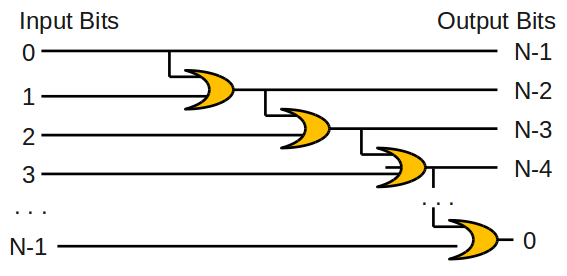
\includegraphics[scale=1.3]{images/or-chain}
	\end{center}
	\caption{The OR Chain Which Calculates the Number of Clock Cycles from the Logical OR of All Frequency Words}
	\label{fig:or-chain}
\end{figure}
Using the resulting clock cycle count, the BIST uses a clock cycle counter to determine when to stop accumulation on an IMP and minimize the error.  Once accumulation has completed the calculation step is triggered and the results are handed off to the calculation circuitry for further processing.

\subsection{On-Chip Calculation Circuit}
\label{sct:onchip}
% Discuss importance of on-chip and how it differs from ORA
% Discuss calculation cordic
% Heavily reference original calculation circuit
% Discuss LOG circuit in joeys thesis verse new circuit which performs all calculations in log
% Discuss how calculations are performed at high-level (so without describing circuitry) for each test and which tests are available
% Linearity, Frequency Response, Spur Search, SNR, NF
The ORA portion of the BIST accumulates the in-phase and out-of-phase components into $DC_1$ and $DC_2$ at the frequency of interest.  Using these values more advanced measurements of special analog characteristics such as linearity, SNR, and NF can be performed.  To do this, $DC_1$ and $DC_2$ must be transformed mathematically into the relative magnitude and phase using Equations \ref{eq:magnitude} and \ref{eq:phase}\cite{joey}.  Traditionally this can be performed off-chip using a mathematical tool such as MATLAB; however, the BIST architecture discussed in this thesis uses an on-chip calculation circuit to perform both of these calculations and to perform multi-measurement tests on-chip\cite{joey}.  First the calculation CORDIC, which converts the $DC_1$ and $DC_2$ values to the magnitude and phase values, will be discussed.

\cite{joey} discusses the original implementation of the calculation circuitry for the BIST approach.  Shown in Figure \ref{fig:joeycalc} the original calculation circuit uses a custom CORDIC developed in \cite{joey} to perform the operations from Equations \ref{eq:magnitude} and \ref{eq:phase} and determine the magnitude and phase from the $DC_1$ and $DC_2$ values; \textit{TC} indicates control signals from the test controller.
\begin{figure}
	\begin{center}
		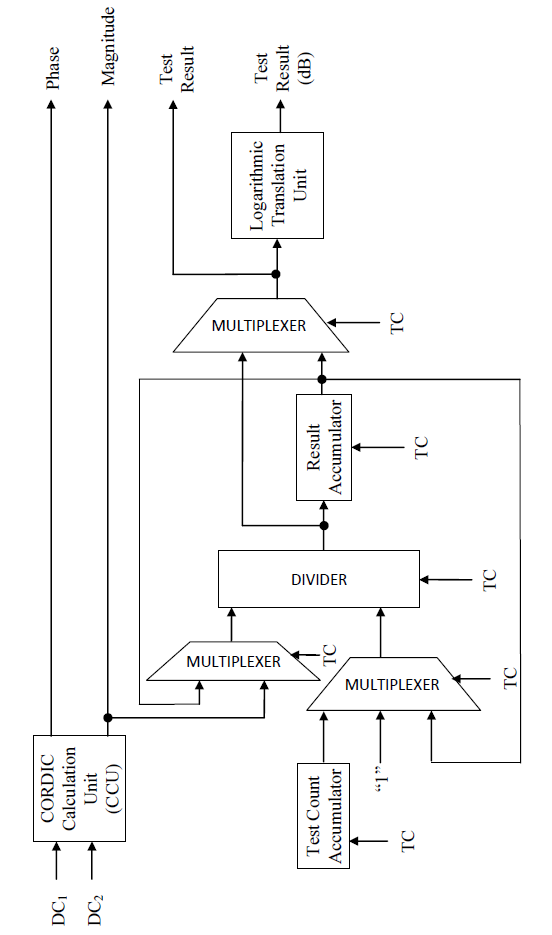
\includegraphics[scale=1]{images/joey-calculation}
	\end{center}
	\caption{Calculation Circuit presented in \cite{joey}}
	\label{fig:joeycalc}
\end{figure}
The CORDIC algorithm, explained in depth in \cite{joey}, is a well-known, low-overhead approach to approximating a number of linear, circular, and hyperbolic functions using successive approximation and inexpensive digital operations such as shift, add, and subtract.  Due to its low area-overhead and convenience, an implementation of this algorithm is used to calculate the magnitude and phase from the $DC_1$ and $DC_2$ values\cite{joey}.  Since it requires successive approximation, the calculation CORDIC requires several clock cycles to complete.  At the end of the approximation the output of the calculation CORDIC is the raw magnitude and phase values which can be read directly and used by the remaining calculation circuitry to perform higher-order analysis\cite{joey}.

The remaining circuitry in the BIST is used for performing multi-measurement tests including measurements of the DUT linearity, SNR, noise figure (NF)\nomenclature{NF}{Noise Figure}, and frequency sweeps. Before discussing each test in detail, it is important to understand that the result of the calculation circuit will be a logarithmic value expressed in decibels.  Decibels (dB)\nomenclature{dB}{Decibel} are a common unit used to represent signal strength.  To simplify the evaluation of measurement output, the calculation circuitry converts the output to decibels as described in Equation \ref{eq:decibel}\cite{joey}.  This operation is performed by the Logarithmic Translation Unit (LTU)\nomenclature{LTU}{Logarithmic Translation Unit} shown at the output in Figure \ref{fig:joeycalc}.  
\begin{equation}
dB = 20 * log_{10}(INPUT)
\label{eq:decibel}
\end{equation}

With the help of the test controller the BIST can perform multi-measurement tests and consequently measure several different important analog characteristics. The first such test measures the linearity of the analog DUT.  The linearity of a system is usually measured by analysis of the third-order inter-modulation point (IP3) using a two-tone test\cite{stroud-automaticlinearity}.  When two tones $f_1$ and $f_2$ are generated and are used to stimulate the DUT, the resulting output frequency will consist of not only $f_1$ and $f_2$ but also the IP3 terms caused by the non-linearity of the DUT.  The output spectrum is shown in Figure \ref{fig:linearityspectrum}.  
\begin{figure}
  \begin{center}
    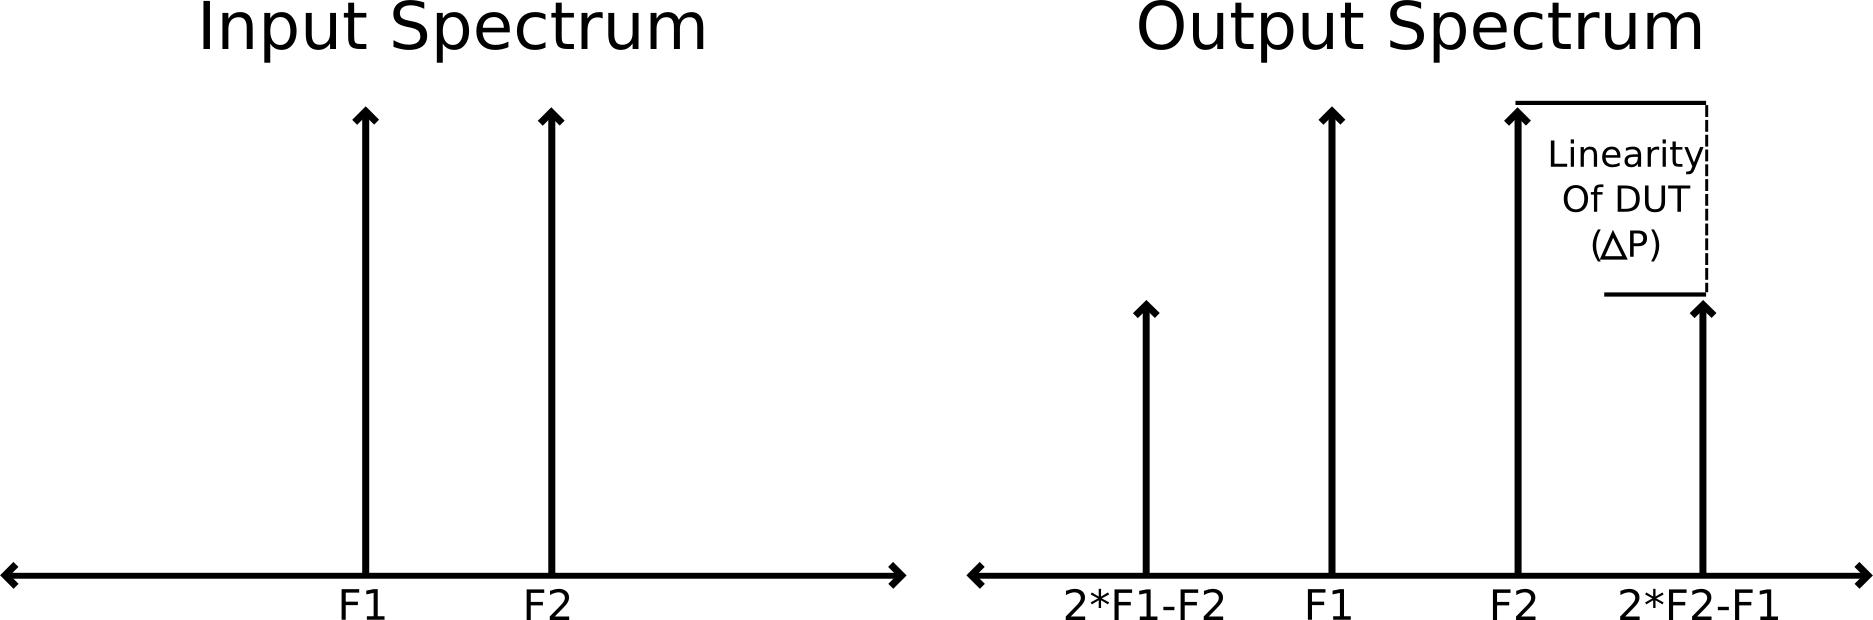
\includegraphics[scale=1]{images/linearity-spectrum}
  \end{center}
  \caption{Input Spectrum v. DUT Output Response for two-tone test}
  \label{fig:linearityspectrum}
\end{figure}
The linearity of a system is the difference in magnitude between the fundamental tone and the IP3 tone; this is often referred to as $\Delta P$\cite{stroud-automaticlinearity}.  When performed in the BIST this requires two measurements.  In both measurements, two frequencies are generated by the DDS $f_1$ and $f_2$.  In the first test the measured frequency is set to $f_2$ and the ORA will accumulate the magnitude and phase of the fundamental frequency $f_2$.  This result is stored in the calculation circuit while a second measurement is performed.  The second measurement measures the IP3 tone at $2*f_2-f_1$\cite{testtime}\cite{jie}.  The resulting magnitude is subtracted from the magnitude of the previous calculation and the result is the $\Delta P$ or linearity of the system.

The frequency sweep test searches a given spectrum for the largest magnitude frequency.  Spurious tones can appear in the spectrum and may negatively affect the output of a DUT.  These tones may be caused by undesired harmonics or due to other issues such as clipping.  It is often required to minimize spurious output and therefore it may be beneficial to measure the magnitude and location of spurious tones in the output of the DUT\cite{joey}.  To perform a frequency sweep no fundamental frequency is generated by the DDS.  To begin the test the frequency of interest $f$ is set to a starting frequency $f_s$ and the magnitude measured.  This magnitude is stored in the calculation circuitry while $f$ is incremented by a predetermined amount $f_{inc}$.  A new measurement will be made at the new frequency of interest $f$ and the magnitude compared to the previously recorded magnitude.  If the new magnitude is greater than the previously stored magnitude, the existing stored values are replaced with the new frequency word and magnitude.  This process will repeat for the number of samples specified.  The result of the test will be the magnitude and frequency word of the largest magnitude spur located in the measured bandwidth\cite{joey}.  In a special case, if $Samples = 0$ only a single frequency's magnitude is measured.  This allows for the frequency response of the DUT to be measured at the specified frequency.  This test can be repeated with a fundamental tone supplied by the DDS and swept through the spectrum to measure the frequency response of the DUT over the specified bandwidth\cite{stroud-automaticlinearity}.

Signal-to-Noise ratio (SNR) and noise figure (NF) are important characteristics of an analog system.  SNR measures the power of the signal of interest in comparison to the average power of the noise in the system over a specified bandwidth.  NF measures the amount of noise and signal degradation added to the system by the DUT by measuring the SNR at the input to the DUT $SNR_{in}$ and comparing it to the SNR at the output of the DUT $SNR_{out}$.  The formulas for these calculations are given in Equations \ref{eq:snr} and \ref{eq:nf} respectively\cite{stroud-nf}.
\begin{equation}
SNR = \frac{Signal\ Power}{Average\ Noise\ Power}
\label{eq:snr}
\end{equation}
\begin{equation}
NF = \frac{SNR_{in}}{SNR_{out}}
\label{eq:nf}
\end{equation}
The BIST can directly perform these tests and measure both of these characteristics.  When performing a SNR measurement the BIST first measures the magnitude of the fundamental signal and stores it.  The next measurement begins at the starting frequency of the bandwidth of interest, $f$ and measures the magnitude.  This measurement is repeated for a predetermined number of samples and the result of each measurement is accumulated in the calculation circuit.  For each repetition the measured frequency $f$ is incremented by a constant $f_{inc}$ specified by the user.  After the specified number of samples has been taken, the accumulated noise power is divided by the number of samples to obtain an average noise power as shown in Equation \ref{eq:noisepower}, where $f_s$ is the starting frequency, $Samples$ is the number of noise samples to take, and $f_{inc}$ is the constant frequency value by which $f$ is incremented.
\begin{equation}
Average\ Noise\ Power =  \frac{\sum_{f=f_s}^{f_s+Samples*f_{inc}} |f|}{Samples}
\label{eq:noisepower}
\end{equation}
After the average noise power is calculated the original signal magnitude is divided by the noise power to obtain the SNR ratio shown in Equation \ref{eq:snr}.  The calculation for NF is very similar.  When performing a NF test the $SNR_{in}$ is calculated by bypassing the DUT (using the previously discussed bypass path) and then divided by the result of a second SNR test $SNR_{out}$ calculated using the standard loopback path.  The result is the NF ratio of the DUT\cite{stroud-nf}.

While the general principals and methods employed by the calculation circuit described in \cite{joey} are still used, improvements to this circuit have been made in the BIST studied in this thesis.  Like the previous calculation circuit it uses the same calculation CORDIC based on the design by \cite{joey} to convert the $DC_1$ and $DC_2$ values to their magnitude and phase representations.  Unlike the previous circuit, the LTU has been moved to the front of the circuit so that all operations are performed in the logarithmic domain.  The divider was replaced by a subtractor as division is performed via subtraction in the log domain.  Coupled with other improvements, the new circuit allows for faster operation and a large reduction in area and power (approximately 33\%).

\subsection{Summary}
% Communication mechanism for BIST
% High-level overview of the SPI
% Summarize the tests possible etc.
\label{sct:bkgsum}
With an understanding of the TPG, ORA, and calculation circuitry of the BIST, the last important aspect of the BIST is how it is controlled and observed (recall that Section \ref{sct:whytest} states that controllability and observability directly influence the testability of a circuit).  Excluding a run signal and the ADC inputs, the majority of the BIST is controlled via a Serial Peripheral Interface (SPI)\nomenclature{SPI}{Serial Peripheral Interface} interface.  An overview of this SPI interface is important to understanding the BIST model.  The SPI input to the BIST consists of an 88-bit SPI word which includes four 15-bit frequency words $FW_1$ through $FW_4$, the number of samples, and a test control word (TCW)\nomenclature{TCW}{Test Control Word} specifying which test to run.  $FW_1$ and $FW_2$ always control the two frequencies generated by the BIST DDS circuitry.  $FW_3$ and $FW_4$ have different meanings depending on the test run and are shown in Table \ref{tbl:fw34}.  
\begin{table}
  \caption{FW3 and FW4 Meanings}
  \begin{center}
    \begin{tabular}{|l|l|l|}
      \hline
      Test Type & Frequency Word 3 ($FW_3$) & Frequency Word 4 ($FW_4$) \\ \hline
      Linearity & IP3 Frequency & Unused \\ \hline
      Frequency Sweep & Starting Frequency $F_s$ & Increment Constant $F_{inc}$ \\ \hline
      SNR \& NF & Starting Frequency $F_s$ & Increment Constant $F_{inc}$ \\ \hline
    \end{tabular}
  \end{center}
  \label{tbl:fw34}
\end{table}
The number of samples is optional and will only be used when a frequency sweep, SNR, or NF test is being executed as discussed in Section \ref{sct:onchip}.  The TCW includes the test type to run as well as some additional flags including those which optionally select  for the use of the digital loopback or bypass path and a bit to enable the use of the half-IMP accumulation time\footnote{Half-IMP accumulation time causes the BIST to accumulate for half of the number of clock cycles that a test would usually require.  This introduces additional error into the calculation but will greatly decrease test-time for long tests\cite{jie-journal}.  This mode is used extensively for fault simulations to minimize test time.}.  

To read data out of the BIST the same SPI is used.  For a read to occur, a SPI write is performed with the read flag set and must include two address bits.  The address bits are decoded by the test controller and correspond to four different 64-bit words which can be read out of the BIST each containing different calculation data related to the test.  The values retrievable are summarized in Table \ref{tbl:readvals}.  $DC_1$ and $DC_2$ correspond to the in-phase and out-of-phase components of the measured frequency (the contents of the MACs).  The magnitude and phase output is the output of the calculation CORDIC and corresponds to the magnitude and phase of the measured signal (directly calculated from $DC_1$ and $DC_2$).  The final values include values specific to each test.  The ``Spur FW'' value corresponds to the location of the largest spur detected when performing a frequency sweep, the ``Log Result'' represents the result of the test in dB, and finally the ``Noise Floor Value'' represents the average noise power as calculated during a SNR test.
\begin{table}
	\caption{Read Address Values}
	\begin{center}
		\begin{tabular}{|l|l|}
			\hline
			Address & Values \\ \hline
			00 & $DC_1$ \\ \hline
			01 & $DC_2$ \\ \hline
			10 & Magnitude and Phase \\ \hline
			11 & Spur FW, Log Result, Noise Floor Value \\ \hline			
		\end{tabular}
	\end{center}
	\label{tbl:readvals}
\end{table}

In addition to the SPI inputs and outputs, there are a few other important outputs used in simulation.  First there is the DDS output which is the generated tone for the test being executed, there is also a 10-bit test result output which is the result of the test in dB.  Finally, there is a ``Done'' flag used to denote that the BIST has finished performing the test requested and that the results are ready for retrieval via the SPI.

\section{Thesis Statement}
%Prob wanna say something about the loopback path again, since he said to
While these descriptions of the BIST architecture are not a comprehensive operating manual, they are provided to give a background of the circuit so that a basic understanding can be developed by the reader.  The focus of subsequent chapters will shift away from the underlying BIST architecture instead focusing on evaluating the effectiveness of the developed test procedures for achieving a high fault coverage when testing a mixed-signal BIST approach by using the SSA BIST circuit as both a benchmark and for context.  In the next chapter the necessary steps for conversion and verification of the circuit model to ASL is discussed.  In addition the development and verification of fault simulation vectors is presented.  These test vectors utilize the digital loopback path\footnote{The digital loopback path is the loopback path which directly connects the TPG to ORA bypassing any analog circuitry including the ADC and DAC.  It is discussed in Section \ref{sct:MixedSignal} and its effectiveness in testing the digital portion of mixed-signal circuitry is evaluated in more depth in \cite{stroud-analog}} to perform measurements used to exercise the BIST circuitry.  After verifying both the ASL and the test vectors, fault simulations are performed and the resulting fault coverage obtained is evaluated in Chapter 4 before a summary and conclusions are drawn in Chapter 5. 

\chapter{Test Preparation, Development, and Verification}
% Talk about verification of ASL first, then relate it to verification of test vectors second
% Note: one way of verifying ASL is to create the test vectors, run them through AUSIM and modelsim and ensure they match clock cycle for clock cycle
% Talk about iterative process for test vector development (though this is kinda discussed in the next section)
To perform fault simulations using AUSIM several steps must be injected into the development process.  This new work-flow, shown in Figure \ref{fig:designworkflow}, first requires conversion of the circuit model to the ASL netlist format which AUSIM can simulate.  Once converted this netlist must be functionally verified as equivalent to ensure that no errors have been introduced during the conversion process.  This chapter will focus first on the conversion process to ASL and the differences between the ASL and Verilog formats.  Following the conversion process, a method of functionally verifying the ASL netlist is introduced which simplifies the verification process by using the Value Change Dump (VCD)\nomenclature{VCD}{Value Change Dump} format and a VCD Viewer.  Finally using a similar method the development and verification of the test vectors for fault simulation is discussed.  In the case of the SSA BIST, these test vectors consist of a number of different measurements including frequency sweep, frequency response, SNR, NF, and IP3 measurements which will exercise the BIST circuitry during simulation.  These measurements utilize the digital loopback path (the path which bypasses any external circuitry, including the ADC and DAC, and directly connects the output of the TPG to the ORA) to facilitate the testing of the digital portion of the BIST for faults avoiding any interference that could be caused by any external analog circuitry. 
\begin{figure}
  \begin{center}
		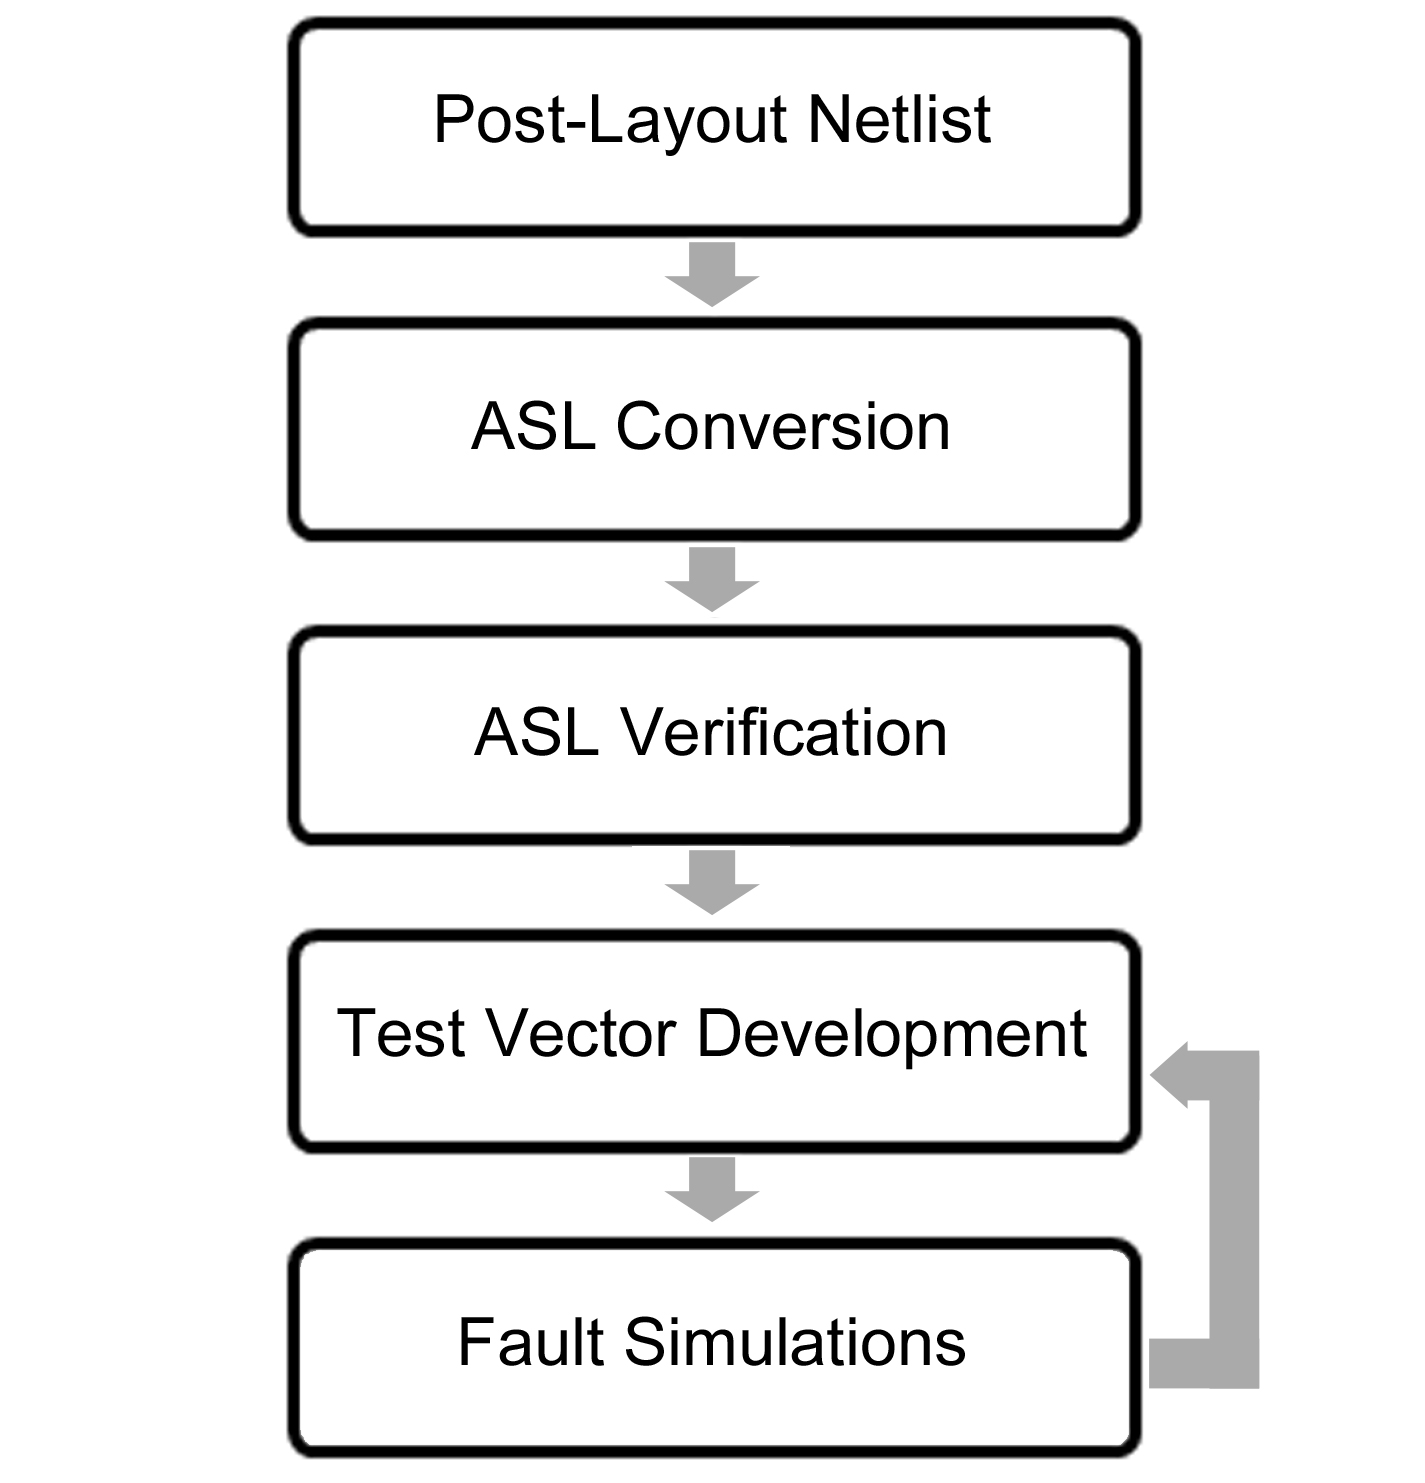
\includegraphics[scale=.1]{images/development-flowchart}
  \end{center}
	\caption{Development Work-Flow}
	\label{fig:designworkflow}
\end{figure}

\section{Converting to ASL}
Behavioral models are commonly written in a high-level hardware description language such as the VHSIC\footnote{VHSIC is an acronym for Very-High-Speed Integrated Circuit\nomenclature{VHSIC}{Very-High-Speed Integrated Circuit}} Hardware Description Language (VHDL)\nomenclature{VHDL}{VHSIC Hardware Description Language} or Verilog.  These languages allow for the behavior of a circuit to be modeled without specifically defining how the behavior is to be implemented in hardware.  For Application Specific Integrated Circuit (ASIC)\nomenclature{ASIC}{Application Specific Integrated Circuit} design this implementation is usually a gate-level implementation of the circuit behavior using technology specific standard cells.  This synthesized netlist is then taken through a place-and-route tool where routing is finalized and a final Verilog netlist is generated\cite{advancedverilog}.  As discussed in Section \ref{sct:designprocess} simulation should ideally be performed using this final implementation of the circuit; unfortunately, AUSIM requires a netlist in the ASL\footnote{See Section \ref{sct:ASL}} format.   To facilitate the rapid simulation of this netlist a tool was developed which allows easy conversion from Verilog to the ASL format.  The VerilogParser tool is written in C\#\cite{csharp} and allows a user to perform fault simulations on any circuit model by synthesizing it to a Verilog netlist then converting it to ASL.  By using the VerilogParser tool, fault simulations using AUSIM can be integrated into the design work-flow easily and efficiently.

As a simple example, a post-layout Verilog netlist of the ISCAS'85 C17 benchmark circuit\footnote{C17 and other ISCAS'85 benchmark circuits can be downloaded from \url{http://courses.engr.illionois.edu/ece543/iscas85.html}} is shown in Table \ref{tbl:c17_verilog_netlist} and its ASL equivalent is shown in Table \ref{tbl:c17_asl_netlist}.  C17 is a small circuit and works well for demonstrating the conversion process as well as the differences between a Verilog and ASL netlist. 
\begin{table}
  \begin{center}
    \caption{C17 Verilog Netlist}
    \begin{tabular}{|l|ll|}
      \hline
      1 & \multicolumn{2}{l|}{\textbf{module} c17(gat1, gat2, gat3, gat6, gat7, gat22, gat23)} \\
      2 & & \textbf{input} gat1, gat2, gat3, gat6, gat7; \\ 
      3 & & \textbf{output} gat22, gat23; \\ 
      4 & & \textbf{wire} gat1, gat2, gat3, gat6, gat7; \\ 
      5 & & \textbf{wire} gat22, gat23; \\ 
      6 & & \textbf{wire} n\_0, n\_1; \\ 
      7 & & AO21\_B g58(.A1 (gat1), .A2 (gat3), .B(n\_1), .Z (gat22)); \\
      8 & & AO21\_B g59(.A1 (n\_0), .A2 (gat7), .B(n\_1), .Z (gat23)); \\
      9 & & AND2\_B g60(.A (n\_0), .B (gat2), .Z (n\_1)); \\ 
      10 & & NAND2\_A g61(.A (gat3), .B (gat6), .Z (n\_0)); \\ 
      11 & \multicolumn{2}{l|}{\textbf{endmodule}} \\ 
      \hline
    \end{tabular}
    \label{tbl:c17_verilog_netlist}
  \end{center}
\end{table}

\begin{table}
  \begin{center}
    \caption{C17 ASL Netlist}
    \begin{tabular}{|l|lll|}
      \hline
      1 & \textbf{CKT}: c17 & \textbf{IN}: gat1 gat2 gat3 gat6 gat7 & \textbf{OUT}: gat22 gat23 ; \\
      2 & \textbf{AO21}: g58 & \textbf{IN}: gat1 gat3 n-1 & \textbf{OUT}: gat22 ; \\  
      3 & \textbf{AO21}: g59 & \textbf{IN}: n-0 gat7 n-1 & \textbf{OUT}: gat23 ; \\  
      4 & \textbf{AND}: g60 & \textbf{IN}: n-0 gat2 & \textbf{OUT}: n-1 ; \\  
      5 & \textbf{NAND}; g61 & \textbf{IN}: gat3 gat6 & \textbf{OUT}: n-0 ; \\ 
      \hline
    \end{tabular}
    \label{tbl:c17_asl_netlist}
  \end{center}
\end{table}
The most significant challenge converting from Verilog to ASL is the difference in the treatment of inputs and outputs of gates.  In Table \ref{tbl:c17_verilog_netlist}, line 7, the instantiation of the AO21 gate is shown.  In Verilog, the gate's inputs and outputs are not designated separately; instead, they use a type of keyword notation which assigns a net to an input or output name.  In this notation, the order of the inputs and outputs does not matter and as such no guarantee is made that the order will be consistent between synthesis tools.  In contrast to this method, Table \ref{tbl:c17_asl_netlist}, line 2, shows the same gate instantiated in ASL.  ASL uses a syntax that declares the inputs and outputs to a gate by position rather than by name and uses the keywords \textit{IN} and \textit{OUT} to clearly separate the input nets from the output nets.  For the translation from Verilog to ASL to be successful, the inputs and outputs of the instantiated gates must be ordered correctly; this includes the ordering of any custom gates defined in an ASL library (library files are discussed in Section \ref{sct:ASL}).   

To solve this problem, several assumptions are made by the VerilogParser tool.  First, it is assumed that in the Verilog netlist elementary logic gates will follow a standard net naming convention where `Z' is the output of the gate.  A similar assumption is made for a Data Flip-Flop (DFF) where the `Q' and/or `QBAR' net names are used for outputs and the `D' and `DBAR' are used for inputs.  More complex logic gates, those gates which are not built-in to AUSIM and require a sub-circuit definition, are treated in a special manner.  With these gates the inputs and outputs are sorted from A-Z when converted.  This means to function correctly each ASL library sub-circuit should have its input and output nets sorted alphabetically.  To determine which nets are inputs and which are outputs, the tool first checks if the instantiated logic gate is defined as a Verilog module.  If a module definition is found, the tool extracts the inputs and outputs of the module to determine how to convert the instantiation to ASL.  Failing this method, the standard rules for elementary logic gates are used where nets prefixed with `Z' and `Q' are assumed to indicate an output while the remaining letters indicate an input\footnote{There are several other net names which are explicitly recognized as outputs such as Sum and Cout}.  Currently there is no method for defining custom translations of the inputs and outputs other than to make modifications to the source code and recompile the tool from scratch.

As a reference Table \ref{tbl:VerilogParserUse} demonstrates how to use the tool on a Verilog netlist.
\begin{table}
  \begin{center}
    \caption{Using the VerilogParser tool to convert a netlist to ASL}
    \begin{tabular}{|l|}
        \hline
        C:$\backslash$Applications$\backslash$ausim\textgreater VerilogParser.exe -aio c17.v c17.asl \\
        Please select the top level module from the list: \\
        -----------------------------------------\\
        0) c17 \\
        Please input the number corresponding to the top level module: 0 \\
        \hline
    \end{tabular}
    \label{tbl:VerilogParserUse}
  \end{center}
\end{table}
The tool works by scanning the Verilog file for module definitions subsequently parsing those modules into an intermediate representation of the circuit.  It then prompts the user to choose which module should be used as the top-level circuit in the ASL netlist before outputting the resulting ASL.  Certain improvements could be made to the parser including automatic detection of the top-level module.  This improvement would require static analysis of the netlist to determine which module is not dependent on any other and as such is suggested for a future version of the tool.  It is also important to note that while the ASL generated by the tool will always be syntactically correct, the tool does not check the validity of the netlist.  It is assumed that any required sub-circuits have already been created and verified in ASL.  

In addition to use in this thesis, this tool has been used to perform other simulations including bridging fault simulations in \cite{james}.  In \cite{james} the VerilogParser tool is used to convert the final post-layout Verilog netlist to the ASL format so that accurate bridging fault simulations can be performed.  The VerilogParser allowed \cite{james} to easily integrate multiple CAD tools which required different netlist formats (in this case a .bench format for automatic test pattern generation using Atalanta, .v for synthesis and place-and-route, and .asl for bridging fault simulations using AUSIM).  The ability to convert between netlist formats easily is clearly advantageous when working with multiple, specialized CAD tools is required.

\section{ASL Verification}
Once the netlist has been converted to ASL using the VerilogParser tool, it must be functionally verified to ensure that it performs identically to the original Verilog circuit model.  This ensures that there were no errors introduced by the conversion process and that the ASL model will behave as expected during simulations.  The most direct way of verifying the ASL netlist is to perform logic simulations using the ASL netlist and subsequently compare the output to the output of logic simulations using the original Verilog model.  If the circuit output of both simulations is identical then the ASL netlist is verified\footnote{It is important to note that a single logic simulation is not enough to verify the ASL model.  Ideally the same logic simulations used to verify the behavior of the Verilog model should be repeated to verify the ASL model.}.  For the SSA BIST test vectors had already been developed to verify the behavioral model of the circuit during the design process.  A subset of these test vectors were converted to the AUSIM vector format and logic simulation performed.  The results were then compared to the simulation results from ModelSim to ensure that they were identical.  Unfortunately the comparison between the AUSIM output and ModelSim can be difficult since the formats used are different.  AUSIM uses a straight-forward text based output format where each line of text represents a test vector applied to the circuit and the corresponding circuit output.  This makes a direct comparison between the output of AUSIM and ModelSim impossible; consequently, a tool was written to convert the AUSIM output to a standard format, the Value Change Dump (VCD) format.  By using a VCD viewer a graphical comparison between the ModelSim and AUSIM output can be performed and the output can be easily analyzed each clock cycle.  This significantly reduces the time required for verification.  The next section provides more information on the VCD format and the conversion process.

\subsection{Value Change Dump File}
The Value Change Dump or VCD format is defined in section 15 of the IEEE 1364-1995 standard for Verilog\cite{verilog}.  Originally created as a light-weight format to dump simulation results for post-processing\cite{verilog}, the VCD format is an industry standard format and is typically used to store logic simulation results in as small of a footprint as possible\cite{verilog}.  In addition as an IEEE standard it is supported in a number of free and commercial viewers which can easily visualize and navigate the underlying simulation data. 

The VCD format compresses simulation results into a smaller footprint by only storing the changes between vectors instead of every vector\cite{verilog}.  While this can make the output of the file less readable it makes it very easy to store large amounts of simulation data and for a viewer to parse and display the file.  An example of a VCD file is shown in Table \ref{tbl:half_adder_vcd}\footnote{It is important to note that while all IO in this example are a single bit, values in a VCD file can be any arbitrary width and in that case operate as a bit-vector.}.  On the right in Table \ref{tbl:half_adder_vcd} is a text description explaining each section of the VCD file.
\begin{table}
	\begin{center}
    \caption{Example VCD File}
		\begin{tabular}{l|l}
			VCD File & Description \\ \hline
			\textbf{\$date} & The date section defines the day\\
			Tuesday, December 07, 2010 & which this file was created \\
			\textbf{\$end} & \\
			\textbf{\$version}
			Generated For ASL2VCD 1.0 & A comment detailing the  \\
			Alex Lusco & version of the application creating this file \\
			\textbf{\$end}	\\
			\textbf{\$comment}	\\
			VCD File & An additional comment section detailing \\
			\textbf{\$end} & information about the file \\
			\textbf{\$timescale} 10ns \textbf{\$end} & Defines the time scale used in this file \\
			\textbf{\$scope} module logic \textbf{\$end} & The simulation scope, particular to the simulation \\
			\textbf{\$var} wire 1 ! A \textbf{\$end} & This section aliases each input with a single ASCII \\
			\textbf{\$var} wire 1 " B \textbf{\$end} & character. For long IO names this shrinks them to a  \\
			\textbf{\$var} wire 1 \# S \textbf{\$end} & single character allowing for the ability to condense \\
			\textbf{\$var} wire 1 \$ C \textbf{\$end} & the dump for large simulations greatly \\
			\textbf{\$upscope} \$end & \\
			\textbf{\$enddefinitions} \$end & End of header \\
			\textbf{\$dumpvars} & Sets the initial value for each input \\
			0!	& Each IO must be set to an initial value here \\
			0"	& The !,",\#, \& \$ characters represent the\\
			0\# & nets aliased in the \$var section\\
			0\$ & \\
			\textbf{\$end} & \\
			\textbf{\#1} & The \#N construct denotes a time step to apply the \\
			1" & following value changes at, in this case at 10ns \\
			1\# & Only nets whose value changed will appear in the time step\\
			\textbf{\#2} & These changes occurred at 20ns \\ 
			1! & \\
			0" & \\
			\textbf{\#3} & These changes occurred at 30ns\\
			1" & \\
			0\# & \\
			1\$ & \\	
			\textbf{\#4} & The end of the simulation, no changes occurred \\		
		\end{tabular}
    \label{tbl:half_adder_vcd}
	\end{center}
\end{table} 
In addition to the file size reduction, the key benefit of conversion to the VCD format is the ability to visualize the output of a logic simulation in one of a number of commercial viewer applications.  For the example in Figure \ref{fig:half-adder-gtkwave} GTKWave was used to visualize the VCD file in Table \ref{tbl:half_adder_vcd}.  GTKWave is a free, open source VCD file viewer for Linux available on-line at \url{http://gtkwave.sourceforge.net}.  In GTKWave each IO is displayed as a waveform which changes over time.  The displayed waveforms can be panned, zoomed and combined.  This functionality alone makes it much easier to verify the output of a complex logic simulation.  
\begin{figure}
	\begin{center}
		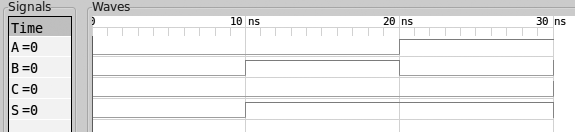
\includegraphics[scale=.4]{images/half-adder-vcd}
	\end{center}
	\caption{VCD File Visualized in the GTKWave Viewer}
	\label{fig:half-adder-gtkwave}
\end{figure}

\subsection{OutToVCD Converter}
The OutToVCD tool is used to convert an AUSIM output file to the VCD format.  It is fairly straight forward to use and greatly simplifies verification of the a test vector set by allowing visual inspection of the results using GTKWave.   An example of using the tool is shown in Table \ref{tbl:outtovcd_example}.
\begin{table}
  \begin{center}
    \caption{Example Usage of ASLToVCD Tool}
    \begin{tabular}{|l|}
      \hline
        C:$\backslash$Applications$\backslash$ausim\textgreater ASLToVCD.exe -g groups.txt c17.out c17.vcd \\
      \hline
    \end{tabular}
    \label{tbl:outtovcd_example}
  \end{center}
\end{table}
This command will convert the logic simulation output of C17 to a VCD file which can be viewed in GTKWave.  The `-g' switch provides a list of outputs which should be concatenated and treated as a bit vector instead of individual bits.  This switch allows for easier verification of multi-bit values.  The tool performs all necessary conversions with no user interaction.

\section{Test Vector Development}
After verifying the ASL, the test vectors to be used for fault simulation must be developed and verified.  This process is similar to the verification of the ASL in that a set of test vectors must be created, logic simulation performed, and the output verified.  Once logic simulation is performed, the output is converted to VCD and analyzed in GTKWave to verify that the test vector set produces the expected output.  Additionally in the case of the SSA BIST, the test vector development process is not automated; instead, an iterative process is required. This process outlined in Figure \ref{fig:testdevproc}, shows the procedure used for developing these test vectors for the SSA BIST.  Initially the test vectors used for fault simulation were manually developed based on an understanding of the underlying BIST architecture. Using knowledge of the BIST architecture, an attempt was made to develop disparate tests which perform measurements that exercise as many different sub-systems of the BIST as possible. 
\begin{figure}
  \begin{center}
		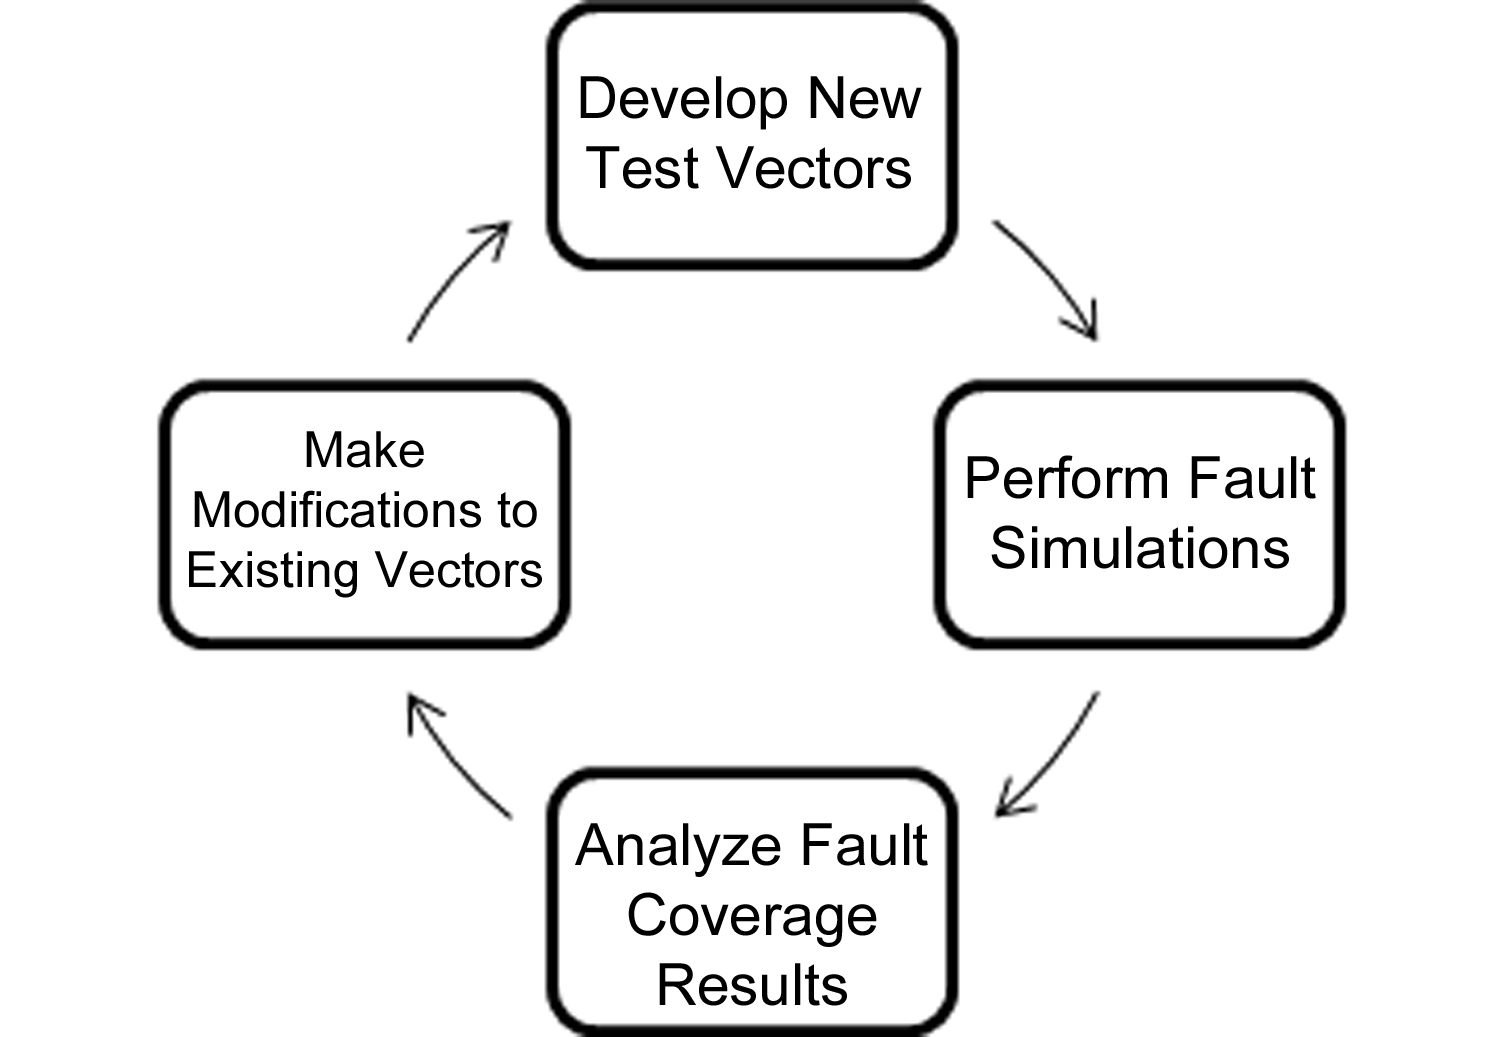
\includegraphics[scale=.15]{images/process-flowchart}
  \end{center}
  \caption{The Test Vector Development Process}
  \label{fig:testdevproc}
\end{figure}
The final measurements used in the fault simulations and the fault coverage obtained is detailed in the next chapter; however, it is important to note that the test procedure shown in Figure \ref{fig:testdevproc} does not allow for the fault coverage of a set of test vectors to be accurately predicted in advance.  Consequently improvements to the test vector set must occur iteratively using feedback from the fault simulations being performed using the current test vector set.  For the SSA BIST, simulations were repeatedly performed using several different measurements and the undetected faults analyzed.  Using this feedback, changes to the initial test vector set were made and new measurements were developed and simulated leading to more analysis and modifications until a suitable fault coverage was obtained. 

\section{Summary}
Using both the VerilogParser tool and the VCD format, ASL conversion and verification can be performed efficiently and quickly.  Once verified the test vector development process can begin and an initial set of test vectors developed.  This set of test vectors is not the final set of vectors used for fault simulation but instead is simulated and the resulting fault coverage analyzed.  Using this analysis, the test vector set can be modified allowing for iterative improvements in fault coverage.  The next chapter discusses the fault simulations and resulting fault coverage achieved using a test vector set developed using this iterative approach.   In addition certain methods are presented which greatly speed up the fault simulations and simplify the analysis of the results.

\chapter{Fault Simulations and Results}
% Introduction To Chapter Structure
% Basic overview
Six measurements were developed using the previously discussed methods and used in fault simulations of the SSA BIST.  These six measurements are the result of efforts to develop a set of measurements which would exercise as much of the BIST circuitry as possible so that a high fault coverage could be obtained.  As previously stated, no tool exists to develop these measurements automatically; consequently, development must occur iteratively with additional measurements added and existing measurements modified based on feedback from fault simulation until a suitable fault coverage is obtained.

In the next section the six measurements are discussed as well as the challenges associated with simulating these measurements.  Following that the results of the fault simulations are analyzed including methods used to determine the individual fault coverage of each measurement, the cumulative fault coverage of all six measurements, and a method used to optimize the ordering of the measurement set.

\section{Performing the Simulations}
% Intro the functional tests which are performed
% Discuss how each test may take different amounts of times, some very long some very short
% How were the tests chosen?  Luck mostly.  Based on our understanding of the underlying architecutre, tests were chosen would exercise as much circuitry of the bist as possible
% Theres no automatic tool for this
% Put a table with each test, the required test time, main circuitry exercised?
Table \ref{tbl:faulttests} shows the details of the six measurements that are used in fault simulations of the SSA BIST.  The first column is the type of measurement (SNR, NF, Linearity (IP3), Frequency Response (FR)\nomenclature{FR}{Frequency Response}, or Frequency Sweep (Sweep)) that is performed during the simulation.  The first and second frequency word columns (\textit{FW1} and \textit{FW2})\nomenclature{FW}{Frequency Word} correspond to frequencies that are generated by the SSA BIST during the test.  The meaning of the \textit{FW3} and \textit{FW4} varies depending on the type of measurement being executed by the BIST and is defined in Table \ref{tbl:fw34}.  \textit{TC Word} is the test control word used for the measurement, this word includes information for the test controller including the measurement type as well as several other measurement flags such as the half-IMP flag\footnote{Discussed in Section \ref{sct:bkgsum}} which halves accumulation time at the expense of measurement accuracy and can greatly shorten the time required for fault simulation.  Measurement accuracy is not a concern for fault simulations since no real signal is being measured; consequently, the half-IMP flag is enabled in most measurements simulated to take advantage of the shortened simulation time.  \textit{Samples} corresponds to the number of frequencies to measure when performing a frequency sweep, SNR, or NF measurement.
\begin{table}
  \begin{center}
    \caption{Simulated BIST Measurements}
    \begin{tabular}{|l|r|r|r|r|r|r|r|}
      \hline
        Type & FW1 & FW2 & FW3 & FW4 & TC Word & Samples & Clock Cycles \\ \hline
        SNR & 1200 & 1400 & 600 & 200 & 13CC & 513 & 103000 \\ \hline
        Long FR & 101 & 101 & 102 & 33 & 0D24 & 0 & 34500 \\ \hline
        Sweep & 1000 & 1500 & 100 & 100 & 0CA4 & 513 & 131500\\ \hline
        IP3 & 3000 & 5000 & 800 & 0 & 070C & 0 & 1050 \\ \hline
        Short FR & 4000 & 6000 & 2000 & 0 & 07A0 & 0 & 900 \\ \hline
        NF & 0CFC & 0AFC & 10FC & 7CCC & 1B60 & 2 & 91601 \\
      \hline
    \end{tabular}
    \label{tbl:faulttests}
  \end{center}
\end{table}
The \textit{Clock Cycles} column is the total number of clock cycles the measurement is simulated and includes SPI writes, reads, and actual measurement accumulation time.  The accumulation time a measurement requires is directly related to the values of its frequency words and is explained in Section \ref{sct:bist-ora}.

Fault simulations were performed for each of the measurements shown in Table \ref{tbl:faulttests}.  For each separate simulation the entire fault list containing 39,497 collapsed faults was used to determine the individual fault coverage of each test.  Using the entire fault list for each test causes a large increase in fault simulation time (recall that Equation \ref{equ:fsimtime} shows that fault simulation time increases as the number of faults simulated increases); however, due to available computing power this was the preferred approach and will be discussed in more detail in the next section.

\subsection{Test Time}
% Discuss the test time taken for each test
% Discuss the advantages of parallel simulation
% Advantages/Disadvantages of running the tests on the entire fault list
% Mention tools used to split fault list and run in parallel on multi-core super computer
% Put the fork script into the appendix (Perhaps a scripts appendix?)
Initially fault simulation was performed using a standard desktop performing very short measurements such as the IP3 measurement from Table \ref{tbl:faulttests}.  This soon proved unfeasible as even fault simulation of the relatively short IP3 measurement took approximately 24 hours to complete.  Realizing that longer tests would prove impossible to complete using this method, an alternative approach was implemented which utilized the Auburn University High Performance Computing Cluster (HPCC)\nomenclature{HPCC}{High Performance Computing Cluster}.  More information can be found about this system at \url{http://www.eng.auburn.edu/admin/ens/hpcc}.  As a general overview the Auburn HPCC consists of four separate computing nodes each with 128 processing cores.  It has 20.48TB of raw storage, 1.536TB of shared RAM, and has an overall performance calculated at 5.735 teraflops\footnote{This and more information about the HPCC is available at the HPCC website}.  By using this system to perform the fault simulations in parallel, simulation time can be drastically reduced.

To take advantage of the HPCC a method was developed to split a given fault list into a number of smaller fault lists each containing the same number of faults.  Each new fault list was copied into its own sub-directory along with a copy of the AUSIM files required to perform the fault simulation including the ASL netlist of the BIST, a test vector file for the measurement being performed, and the output from a previously performed logic simulation.  Once the fault list has been split up and prepared, a job scheduler script was submitted to the HPCC scheduler which requests the required number of processing cores.  Once loaded into the HPCC, this script forks the appropriate number of AUSIM processes (one for each CPU core) and each split fault list is simulated in parallel.  Due to limitations imposed by the HPCC administrator a maximum of only 128 CPU cores could be requested by a single user using the system thus limiting the number of parallel simulations that could be run at a given time to 128\footnote{As shown in Table \ref{tbl:faulttesttime} greater than 128 CPU cores were used in some measurements due to temporary changes in the restriction by the HPCC administrator}.  

Table \ref{tbl:faulttesttime} shows the total CPU time used by each test in hours vs the number of actual hours required to perform the simulation (wall time).  In addition to the original six measurements shown in Table \ref{tbl:faulttests}, an additional simulation is also shown where all six measurements were combined together and run sequentially in a single fault simulation.  Looking at the worst case fault simulation time (the combined simulation), without using the Auburn HPCC for simulation the combined measurement would have take 6072 hours or approximately 253 days to complete! Instead, by splitting it up and running 128 parallel simulations it required only three days to perform.  This speed up provided the flexibility to perform longer measurements without concern for the simulation time.
\begin{table}
  \begin{center}
    \caption{Fault Simulation Test Time}
    \begin{tabular}{|l|l|l|l|l|}
      \hline
      Type & CPUs Used & CPU Time (Hr) & Wall Time (Hr) & Speed Up \\ \hline
      Combined & 128 & 6072 & 74 & x82 \\ \hline
      SNR & 127 & 2018 & 20 & x100 \\ \hline
      Long FR & 25 & 12.5 & .6 & x21 \\ \hline
      Sweep & 384 & 3450 & 28 & x123 \\ \hline
      IP3 & 25 & 8.5 & .5 & x17 \\ \hline
      Short FR & 99 & 609 & 9 & x68 \\ \hline
      NF & 256 & 2544 & 21.7 & x117 \\
      \hline
    \end{tabular}
  \label{tbl:faulttesttime}
  \end{center}
\end{table}

This technique does not come without disadvantages.  First additional development was required to create the methods and techniques used to perform these simulations as no previously work had been done which used the HPCC for fault simulation purposes.  This process involved some trial and error as the HPCC job scheduling system was not well documented and best practices for using the system had to be determined.  Second it can complicate the analysis of the fault simulation results since results are split among a number of different parallel simulations and must be recombined and processed before any results can be determined.  The next section discusses in detail the methods used to calculate both the individual and cumulative fault coverage obtained for the six tests in Table \ref{tbl:faulttests}.

\section{Fault Coverage Results}
% Start with challenges related to recombining data from parallel simulations
% Once combined fault list needs to be analyzed to determine coverage
Once a fault simulation has been completed using the HPCC, the fault coverage results are split amongst separate sub-folders.  In each folder (one for each CPU core which was used in the simulation) there are three files of interest, the detected fault list, the potentially detected fault list, and the undetected fault list.  The first step to determining the fault coverage is to recombine all of these separate fault lists, creating one combined list for each type of fault.  To do this a simple script is used which utilizes the Linux \textit{cat} and \textit{awk} commands to append each of the files together and then remove any blank lines or comments from the output.  The result of this operation is three files (one for each type of fault: detected, undetected, or potentially detected (PDT)\nomenclature{PDT}{Potentially Detected}).  Each of these files contains either the total number of detected, undetected, or PDT faults for this measurement.  By applying Equation \ref{equ:faultcvg} to this data, the fault coverage can be calculated by taking the number of detected faults, adding a percentage of the potentially detected faults, and then dividing by the total number of faults (less any faults which are undetectable).  However, before using Equation \ref{equ:faultcvg} to calculate the fault coverage, an analysis of the PDT fault list is performed so that a more accurate estimate of the likelihood of a potentially detected fault being detected can be formed.

\subsection{Potentially Detected Faults}
% Discuss the filtering of potentially detected faults based on # of detections
% In our case we choose 300 as the cut off
It is common to assume that 50\% of the PDT faults will be detected in a real system and multiple $P$ by $.5$ in Equation \ref{equ:faultcvg}.  This is an easy assumption to make; however, with some simple analysis of the PDT fault list we can do a better job approximately the likelihood of a PDT fault being detected.  

The PDT fault list that AUSIM outputs includes both the fault name and the number of times the fault was potentially detected during simulation.  By making the assumption that a high number of detections of a PDT fault will result in a high likelihood of that PDT fault being detected in a real system, the fault list can be post-processed to mark any PDT faults that fulfill this criteria as detected faults.  When analyzing the fault simulation results of the SSA BIST, there proved to be a large separation between the PDT faults which were detected only a few times and those which were detected a high number of times.  Based on this qualitative data, a threshold of 300 detections was chosen to separate the two categories.  An automated script was then developed to perform this processing, and when run marks any PDT fault which is detected greater than or equal to 300 times as detected.  In the future more research should be done to determine a more quantitative relationship between the number of times a PDT fault is detected verse the likelihood of detecting the fault in real hardware.

\subsection{Undetectable Faults}
As shown in Equation \ref{equ:faultcvg}, any undetectable faults should be excluded from the total number of faults when calculating fault coverage.  Due to optimizations made by the synthesis tools when generating the post-layout Verilog netlist of the SSA BIST, a number of undetectable faults were encountered when performing fault simulations that had to be removed.  These faults occur due to nets which may be tied directly to VDD or GND due to logic minimization performed by the synthesis tool.  Unfortunately AUSIM has no direct method of representing a net tied to VDD or GND so a slightly modified sub-circuit is used.  
\begin{figure}
  \begin{center}
		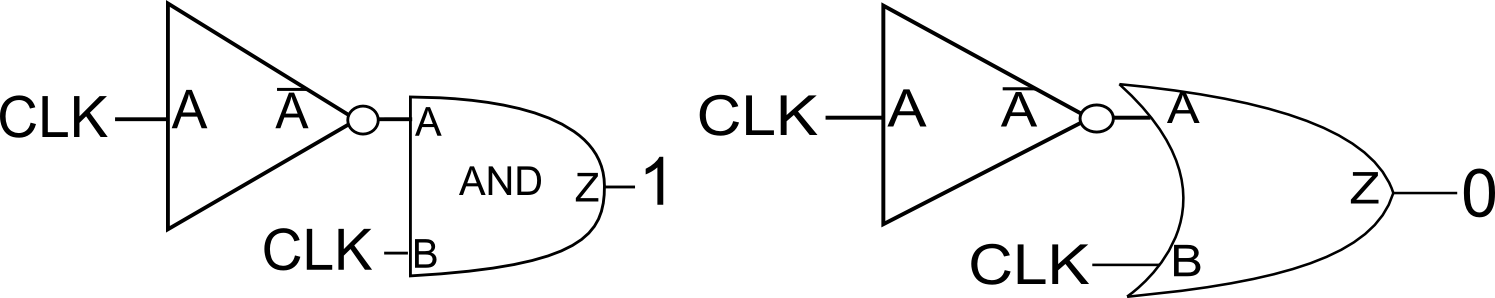
\includegraphics[scale=.9]{images/vdd-gnd}
  \end{center}
  \caption{Method used to Represent Connection to VDD and to GND in AUSIM}
  \label{fig:ausim_undetectable}
\end{figure}

Shown in Figure \ref{fig:ausim_undetectable} an AND gate and inverter are used to generate a value which is always logic `0' (GND) and an OR gate and an inverter are used to generate a value which is always logic `1' (VDD).  In both of these circuits, CLK is used as the input net; however, any net can be used that is convenient.  Regardless of the input value these circuits will always generate a logic `0' and logic `1' respectively.  While these two sub-circuits work well to solve the issue during conversion and logic simulation, they each introduce an additional undetectable fault which must be accounted for during fault simulation.  In the case of the AND circuit, any net stuck-at `0' is undetectable since the output of the AND gate is always a logic `0'.  Likewise in the case of the OR gate, any net stuck-at `1' is undetectable since the output of the OR gate is always a logic `1'.  After conversion to ASL, the SSA BIST contained approximately 14 undetectable faults due to these circuits.  These faults were removed via an automated script from the fault list and not including in any of the fault coverage calculations.

\subsection{Overall Fault Coverage}
% Discuss fault coverage of each test
% Discuss techniques used to determine unique faults detected vs unique potential faults
Each of the six measurements in Table \ref{tbl:faulttests} were simulated and the results recorded.  Each test was simulated against the entire list of 39497 faults.  The individual fault coverage of each test is shown in Table \ref{tbl:faultresults}.  The \textit{Raw Detected} and \textit{Raw Potentials} columns are the number of faults reported by AUSIM; however, as discussed in the previously any potentially detected faults which were detected greater than 300 times were marked as detected.  This is shown in the \textit{Detected} column which contains the number of raw detected faults plus the number of PDT faults which were detected greater than 300 times and in the \textit{Potentials} column which contains the number of raw PDT faults less any PDT faults detected greater than 300 times.  The overall fault coverage is in the \textit{Coverage} column and is calculated using Equation \ref{equ:faultcvg}.  This coverage is calculated using the modified detected and PDT fault numbers and assumes a 50\% probability of detecting any remaining PDT faults (those which were potentially detected less than 300 times).
\begin{table}
  \begin{center}
    \caption{Individual Fault Coverage Results}
    \label{tbl:faultresults}
    \begin{tabular}{|l|l|l|l|l|l|}
      \hline
      Type & Raw Detected & Raw Potentials & Detected & Potentials & Coverage \\ \hline
      SNR & 27310 & 3387 & 30570 & 127 & 77.55\% \\ \hline
      Long FR & 25526 & 3337 & 28313 & 551 & 72.38\% \\ \hline
      Sweep & 25256 & 3406 & 28419 & 243 & 72.26\% \\ \hline 
      IP3 & 22122 & 3102 & 24994 & 230 & 63.57\% \\ \hline
      Short FR & 20617 & 3456 & 23815 & 258 & 60.62\% \\ \hline 
      NF & 27883 & 3354 & 31007 & 230 & 78.80\% \\ 
      \hline
    \end{tabular}
  \end{center}
\end{table}
It is important to note that Table \ref{tbl:faulttests} is the individual fault coverage of each measurement and that further processing must be done to obtain the cumulative fault coverage of all measurements.  

To determine the cumulative fault coverage all measurements must be combined and the unique set of both detected and potentially detected faults extracted.  Once extracted the unique PDT fault list is analyzed and PDT faults which are detected more than 300 times are removed and marked as detected.  The final fault numbers are then used with Equation \ref{equ:faultcvg} and the final cumulative fault coverage can be determined.  In the case of the SSA BIST the raw, cumulative number of detected faults was 31639 and the raw, cumulative number of potential faults was 3521.  After filtering out the potential faults which were detected greater than 300 times, the number of detected faults rose to 34831 and the number of potential faults became 360.  This results in a cumulative fault coverage of 88.64\%.  

To obtain a better understanding of which measurements are most effective at detecting faults in the SSA BIST, it is beneficial to determine the incremental fault coverage each test contributes to the cumulative fault coverage total of 88.64\%.  By determining the number of additional unique faults each measurement detects, the measurements can be ranked and ordered by highest incremental improvement in fault coverage.  This has a number of practical implications.  First it can be used to determine which measurements are providing the most benefit to the cumulative fault coverage.  Measurements which provide only a minor increase in the cumulative fault coverage may need to be reworked or replaced.  Unfortunately as the cumulative fault coverage becomes higher, it becomes increasingly more difficult to obtain substantial improvements in fault coverage with each additional measurement.  Secondly if the measurements are ordered from the highest to least number of unique detected faults then the time required to perform a combined fault simulation (similar to the one performed in Table \ref{tbl:faulttesttime}) of all measurements can be minimized.  This decrease in time occurs due to fault dropping of detected faults (Section \ref{sct:faultsim}) causing a decrease in the number of faults simulated for the entire length of the simulation.  In addition when verifying an actual hardware implementation using this test procedure, measurements which detect the most faults will be performed first increasing the likelihood that a fault is detected early in the test sequence.  This will shorten the overall verification time as unnecessary measurements are not run.

To determine the optimum measurement order a script was developed which analyzes the detected fault lists from an arbitrary number of simulated measurements.  First the measurement with the highest number of detected faults is selected as the initial measurement to be run.  Starting with this initial list of detected faults, the measurement which provides the highest incremental improvement of fault coverage is then selected to be run next.  This is repeated until the optimum test order is determined.  

Figure \ref{fig:cumulativefault} shows the optimum ordering of the six measurements and the individual and cumulative fault coverage gain for each measurement.  As discussed previously any potentially detected faults detected greater than 300 times are included in the number of detected faults.
\begin{figure}
  \begin{center}
		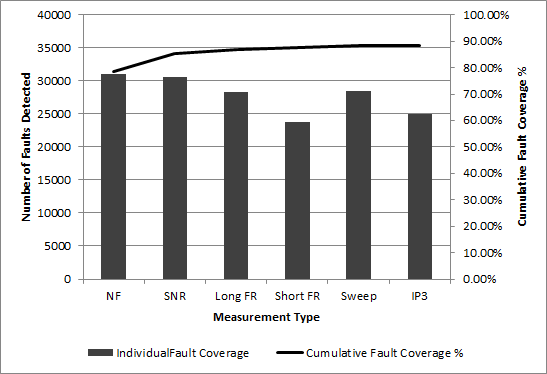
\includegraphics[scale=.9]{images/faultcvg-graph}
  \end{center}
  \caption{Individual Fault Coverage vs Cumulative Fault Coverage Percentage}
  \label{fig:cumulativefault}
\end{figure}
As shown in the graph the cumulative fault coverage rises little after the first three measurements have been performed (NF, SNR, Long FR).  In fact these first three measurements detect a total of 34335 faults, a cumulative fault coverage of 86.93\%.  The remaining measurements only detect an additional 623 faults. 

After determining the optimum order to perform the measurements, a fault simulation was performed where all measurements were executed sequentially in a single fault simulation and the fault coverage obtained verified.  This combined fault simulation required a total of 1,011,900 test vectors to be simulated requiring approximately 673 hours of CPU time.  As shown in \ref{tbl:faulttesttime} this time was reduced down to approximately 74 hours using the parallel fault simulation techniques discussed previously.  As expected the fault coverage obtained in the combined test was 88.64\% matching the coverage calculated from the individual measurement simulations.

\section{Experimental Results}
The six measurements developed using this test procedure have successfully been used to verify a hardware implementation of the SSA BIST discussed in this thesis.  Using the digital loopback path of the SSA BIST, each of the six measurements was executed on each SSA BIST chip and the output compared to the previously performed logic simulations.   This entire process was automated and performed at the system clock speed of 80MHz.  Approximiately 500,000 clock cycles are required to perform all six measurements which correlated to a test time of a little under 10ms.  If during the testing process a chip did not produce the expected results after performing a given measurement then it was considered faulty.  Using this procedure several chips were identified as faulty after failing to return the correct values.  In addition in one specific case the location of the fault was able to be diagnosed based on analysis of the invalid BIST results.  The successful use of this test procedure to verify actual hardware proves that this method is an efficent and viable method for the fault-free verification of mixed-signal systems and in some cases can aid in fault diagnosis.

The next chapter will summarize these findings and address some of the implications of the fault coverage obtained as it relates to the observability and testability of the BIST approach.  Opportunities for improvements to the BIST approach will be briefly discussed including some simple modifications to the underlying BIST architecture which may result in an increase in fault coverage by improving the testability of the BIST.

\chapter{Analysis and Summary}
% Reasons fault coverage were low, limited signal generation capabilities, some registers not observable (samples)
% Mention possible improvements that should be performed and expected area increase etc, clipping, shifting for attenuation, disabling of spur stuff (maybe not)
% This thesis recap... needs to say an awesome summary of everything, did it work? (yes)
% Advantages over DFT (area, etc.. maybe this hsould go in chapter 3?... Chapter 2?)
While a cumulative fault coverage of almost 89\% is an excellent starting point it is not as high as might be desired.  To work towards a higher fault coverage it would be beneficial to identify the key areas not covered by the current test vector set and other sub-circuits of the BIST which are not easily testable or observable.  This section starts by analyzing the fault coverage obtained and looking at areas of the SSA BIST which are not easily testable or observable.  After identifying these weak areas, several design modifications to the BIST are explored which may allow an increase in the cumulative fault coverage that is obtainable.  Finally an overview of this thesis is provided and a summary is given of the work completed.

\section{Fault Coverage Analysis}
By analyzing the faults which were detected and undetected by the fault simulations performed in Chapter 4, a better understanding of the testability of the SSA BIST can be obtained.  Table \ref{tbl:faultsubsystems} shows the fault coverage of several of the BIST sub-systems obtained by running the six previously discussed measurements\footnote{The Fullswing Power and Spur Calibration sub-systems are circuitry which normalize the result of an accumulation when performing a single frequency response measurement}. Each major sub-system of the SSA BIST is identified and the approximate fault coverage of the sub-system is given.  As shown in the table, several areas of the BIST including the DDS, MACs, and reference CORDIC have greater than 95\% fault coverage.  
\begin{table}
  \begin{center}
    \caption{Fault Coverage of BIST Sub-Systems}
    \label{tbl:faultsubsystems}

    \begin{tabular}{|l|r|r|}
      \hline
      Subsystem & Total Faults & Coverage \\ \hline
      DDS & 4995 & 99.7\% \\ \hline
      Fullswing Power & 438 & 70.09\% \\ \hline
      LOG Calculation & 11621 & 81.06\% \\ \hline
      ORA Accumualtors & 10608 & 98.37\% \\ \hline
      Reference CORDIC & 3977 & 95.22\% \\ \hline
      Spur Calibration & 660 & 71.06\% \\ \hline
      Test Controller & 1829 & 85.27\% \\ \hline
      SPI Interface & 4259 & 81.71\% \\
      \hline
    \end{tabular}
  \end{center}
\end{table}
The high fault coverage of these sub-systems is not particularly suprising as each is extensively exercised by each measurement performed.  Unfortunately several of the other sub-systems are not as easily testable.  Particularly the calculation circuitry, some related normlization circuitry, portions of the test controller, and the external SPI interface have a relatively low fault coverage compared to other sub-systems.  To improve the overall fault coverage obtained, several improvements to the BIST are proposed and analyzed which improve the testability of the LOG Calculation, Test Controller, Spur Calibration, and Fullswing Power sub-systems.  Due to design restrictions it is not possible to make modifications to the SPI interface and it was excluded from consideration.

\section{Fault Coverage Improvements}
By analyzing the logic simulation results of the six measurements performed several weaknesses were identified in the testability of the SSA BIST.  The first major weakness determined was that the possible measurable signals was limited.  When simulating or performing these measurements the digital loopback path is used.  Also any signals to be measured must be generated by the DDS. Unfortunately the digital loopback path is a purely digital path; consequently, there is no noise introduced by components nor is there any noise inherient to the path or signal loss possible.  This limits the possible signal magnitudes that can be measureds to two possible options.  The first possible magnitude that can be measured is the maximum power sine wave generated by the DDS.  The second possible magnitude that can be measured is when a point in the spectrum is measured where no signal is located; this corresponds to a zero magnitude signal (since there is no noise in a digital circuit).  Since only two magnitude signals can be produced this seriously limits the bits exercised in the calculation circuitry as well as the fullswing power and spur calibration circuitry. 

A second major weakness is also rooted in the pure digital nature of the digital loopback path.  In this case the digital loopback path always has maximum possible linearity since it is a digital path.  Since no clipping of the generated DDS signals can occur and there is no noise introduced into the system, any linearity measurement preformed by the BIST will always return the maximum measurable linearity value.  This is an issue as it limits the amount the calculation circuitry can be exercised and subsequently tested potentially lowering the possible fault coverage achievable.

Finally the test controller has fairly low test coverage though the reasoning behind this isn't quite as easily attribute to a single issue.  For one this is likely due to the measurement set not poerply exercising some of the measurement options available.  Unfortunately this is difficult as some measurement options cannot be performed when in loopback mode (such as usage of the bypass path or using the certain preset circuitry\footnote{The preset circuitry holds a number of predetermined BIST measurements hard-coded into the model and selectable via the SPI and external pins.  These measurements each include the test type and options not allowing for the digital loopback path to be used.  This effectively prevents this circuitry from being tested.}).  

An additional measurement option that is difficult to observe is the samples register.  The samples register controls the number of samples that are taken when performing an SNR, Frequency Sweep, or Noise Figure measurement.  This register is a 10-bit register allowing upto 1024 samples to be taken in a single measurement.  To fully verify that this register is fault-free a measurement must be performed which takes a minimum of 513 samples.  Performing a measurement that takes 513 samples requires a lengthy simulation time.  Regardless of the simulation time a measurement that does exactly this is performed as part of the six measurements simulated in Chapter 4; however, if this register was easier to observe it would not require that such a long measurement be included in the test vector set potentially allowing for a more effective measurement or even multiple shorter measurements to be performed in its place.

To address these issues, four main improvements to the SSA BIST were suggested and subsequently simulated to determine if any improvement in fault coverage was obtained.  These four improvements incurred little area penalty (\textless 2\%) and include:
\begin{itemize}
  \item The option to disable certain output normilzation circuitry when performing frequency response measurements
  \item The ability to perform a shift operation on the DDS output to attentuate the signal so that multiple magnitude signals could be produced and measured
  \item The ability to purposely clip the DDS output within the digital loopback path introducing harmonics that can be measured in linearity tests
  \item Allow the testing of the preset circuitry by forcing any preset measurement to be performed using the digital loopback path
  \item Allow the samples register to be read out via the BIST SPI interface 
\end{itemize}
The original six measurements discussed in Chapter 4 were resimulated using the modified BIST architecture and the fault coverage recorded.  Following the original six measurements four additional measurements were developed using the test procedure outlined in Chapter 3.  Each of these four measurements utilized the improvements made to the BIST circuit to determine the effectiveness of the discussed improvements.  The four newly developed measurements are:
\begin{itemize}
  \item A frequency response measurement with a single sample which uses the shift functionality to reduce the magnitude of the generated DDS signal
  \item A linearity test which utilizes the clipping ability to introduce non-linearity into the digital loopback path
  \item A SNR measurement with 513 samples which uses the clipping and shifting to modify the DDS signal measured
  \item A frequency response measurement that is stored in the preset circuitry of the BIST and utilizes the override flag to run using the digital loopback path
\end{itemize}

The fault coverage of all ten measurements is shown in Figure \ref{fig:newfaultcvg}.  Unfortunately as shown in the figure, the final fault coverage of all tests proved to be only 90.00\% approximately a 1.5\% improvement.  While this does not invalidate the improvements made to the BIST loopback (some fault coverage increase was obtained), it does show that the fault coverage is not explictly limited by the factors discussed.  This likely means that future improvements to fault coverage will come via iterative improvements to the measurement set.  This also likely indicates that it will be difficult to acheive major increases in fault coverage in future iterations and any progress made will require adding additional measurements to the measurement set with only small increases in the number of detected faults (on the order of a few hundred faults).
\begin{figure}
  \begin{center}
		
\includegraphics[scale=.7]{images/placeholder}
  \end{center}
  \label{fig:newfaultcvg}
  \caption{Fault Coverage of New Measurement Set using BIST Improvements}
\end{figure}

\section{Conclusions}
Unfortunately approximiately 90\% fault coverage is as high as was achievied using the measurement set developed in this thesis.  Even with the improvements proposed and implemented in the BIST the gain realized was minimal.  This is not to say that the maximum fault coverage achievable is limited to 90\% though it is possible that it may be near the upper limit that can be achieved with as little as six measurements.  Certain areas of the BIST are impossible to test while using the digital loopback mode in simulation and these areas will impose a limit on the fault coverage achievable.  These areas are mostly related to external circuitry such as external run control and the bypass and ADC paths.  These circuits cannot be tested when using the digital loopback mode and SPI.  Future research should determine the number of faults attributed to untestable paths and what fault coverage could be achieved after removing these faults.

Regardless of the marginal improvement in fault coverage provided by the changes to the BIST, a fault coverage of almost 90\% was obtained using the test procedure outlined in this thesis.  In this procedure a method was presented to iteratively develop a set of measurements to be executed by a mixed-signal BIST system to test itself for faults.  A conversion process is outlined which converts any post-layout verilog model to the ASL format (and verifies the correctness of the ASL model) so that fault simulation can be performed and the fault coverage of developed measurements evaluated.  Using the SSA BIST as a benchmark, this procedure has shown that by utilizing the digital loopback, an set of measurements can be created which allow a mixed-signal BIST to effectively test itself for faults without the need for external test equipment and without requiring dedicated testing circuitry such as scan chains.  

There are several hurdles when using this approach as compared to other testing approaches such as scan.  First it does require a significant amount of time to iteratively develop and simulate the measurement set used when testing the mixed-signal BIST.  There is no automated tool that can develop the test vector set and some trial and error is needed to develop a test vector set which yields a sufficently high fault coverage.  Second as discussed earlier it may prove difficult to acheive the highest levels of fault coverage (\textgreater 95\%) due to some portions of the BIST being untestable such as external run pins and external loopback paths.  These types of circuitry (and related control circuitry) cannot be tested in a digital loopback mode and could potentially be the source of a number of undetected faults limiting the maximum fault coverage obtained in the SSA BIST. 

Regardless of these disadvantages, this test procedure does have a significant number of advantages compared to other methods.  It is circuit agnostic requiring only a post-layout Verilog model for the conversion process and a digital loopback path for testing purposes.  So while development of the test vector set must occur iteratively, it can be fine-tuned for the specific architecture being tested and intuitively evolved.  In addition by utilizing this method of testing no performance or area penalty is incurred in the circuit.  All testing is performed using the digital loopback path and no dedicated test circuitry must be inserted into critical path ways.  This also means that testing can be performed without external equipment and at system speed.  As stated in Chapter 4 with a sufficently high system clock speed, the actual testing of real hardware using the simulated measurement set can be performed very quickly and efficently.  

% Bibliography
\begin{thebibliography}{99}

\bibitem{stroud} C. Stroud, \textit{A Designer's Guide to Built-In Self-Test}. Kluwer Academic Publishers, 2002.

\bibitem{itrs} \textit{The International Technology Roadmap for Semiconductors: 2009 Edition - Test \& Test Equipment}, Semiconductor Industry Association, San Jose, CA.

\bibitem{zorian} Y. Zorian, ``Testing the Monster Chip,'' \textit{IEEE Spectrum}, vol. 37, no. 7, pp. 54-60, 1999.

\bibitem{ungar} L. Ungar and T. Ambler, ``Economics of Built-In Self-Test,'' Proc. \textit{IEEE Design \& Test of Computers}, vol. 18, no. 5, pp. 70-79, 2001. 

\bibitem{syschip} L. Wang, C. Stroud, N. Touba, Eds., \textit{System On Chip Test Architectures}. Elsevier, 2008.

\bibitem{milor} L. Milor and V. Visvanathan, ``Detection of Catastrophic Faults in Analog Integrated Circuits,'' Proc. \textit{IEEE Transactions on Computered-Aided Design of Integrated Circuits and Systems}, vol. 8, no. 2, pp. 114-130, 1989.

\bibitem{stroud-analog} C. Stroud, P. Karunaratna, and E. Bardley, ``Digital Components for Built-In Self-Test of Analog Circuits,'' Proc. \textit{IEEE 10th ASIC Conference and Exhibit}, pp. 47-51, 1997.

\bibitem{ausim} C. Stroud, ``AUSIM: Auburn University SIMulator - version 2.0,'' Dept. of Electrical \& 
Computer Engineering, Auburn University, July 7, 2003.

\bibitem{asl} C. Stroud, ``ASL: Auburn Simulation Language,'' Dept. of Electrical \& Computer
Engineering, Auburn University, July 7, 2003.

\bibitem{verilog} ``IEEE Standard Hardware Description Language Based on the Verilog(R) Hardware Description Language,'' IEEE Std 1364-1995, 1996.

\bibitem{analogfaults} L. Milor, V. Visvanathan, ``Detection of Catastrophic Faults in Analog Integrated Circuits,'' \textit{IEEE Transactions on Computer-Aided Design of Integrated Circuits and Systems}, vol.8, no.2, pp.114-130, 1989.

\bibitem{analogosc} K. Arabi and B. Kaminska, ``Oscillation-Test Strategy for Analog and Mixed-Signal Integrated Circuits,'' Proc. \test{IEEE VLSI Test Symposium},  1996, pp. 476-482.

\bibitem{faultdiagnosis} V. Yarmolik, \textit{Fault Diagnosis of Digital Circuits}. John Wiley & Sons, 1990.

\bibitem{analogmixedtest} B. Vinnakota, \textit{Analog and Mixed-Signal Test}. Prentice Hall, 1998.

\bibitem{defectforcmos} M. Sachdev, \textit{Defect Oriented Testing for CMOS Analog and Digital Circuits}.  Kluwer Academic Pub, 1998.

\bibitem{stroud-bridging-physical} C. Stroud, J.Emmert, J. Bailey, D. Nickolic and K Chhor, ``Bridging Fault Extraction from Physical Design Data for Manufacturing Test Development'', Proc. \textit{IEEE International Test Conference}, 2000.

\bibitem{stroud-bridging} J.M. Emmert, C. Stroud, J.R. Bailey, ``A New Bridging Fault Model For Accurate Fault Behavior,'' Proc. \textit{IEEE Automatic Test Conference}, pp 481-485, 2000.

\bibitem{parallelflts} D.G. Saab, I.N. Hajj, J.T. Rahmeh, ``Parallel-Concurrent Fault Simulation,'' Proc. \textit{IEEE International Conference on Computer Design: VLSI in Computers and Processors}, pp.298-301, 1989.

\bibitem{advancedverilog} C. Last, \textit{Advanced Digital Design The Verilog HDL}.  Prentice-Hall, 2004.

\bibitem{testtime} J. Qin, C. Stroud, F. Dai, ``Test Time of Multiplier/Accumulator Based Output Response Analyzer in Built-In Analog Functional Testing,'' Proc. \textit{41st Southeastern Symposium on System Theory}, pp.363-367, 15-17 2009.

\bibitem{noisefigure} J. Qin, C. Stroud, F. Dai, ``Noise Figure Measurement Using Mixed-Signal BIST,'' Proc. \textit{IEEE International Symposium on Circuits and Systems}, pp.2180-2183, 27-30 2007.

\bibitem{basessa} F. Dai, C. Stroud, and D. Yang, ``Automatic Linearity and Frequency Response Tests with Built-in Pattern Generator and Analyzer,''  \textit{IEEE Transactions on VLSI Systems}, vol. 14, no. 6, pp. 561-572, 2006.

\bibitem{csharp} Microsoft. The C\# Language. Visual C\# Developer Center. [Online] \url{http://msdn.microsoft.com/en-us/vcsharp/aa336809.aspx}.

\bibitem{jie} J. Qin, ``Selective Spectrum Analysis (SSA) and Numerically Controlled Oscillator (NCO) in Mixed-Signal Built-In Self-Test,'' Doctoral Dissertation, Auburn University, 2010.

\bibitem{joey} G. Starr, ``Built-in Self-Test for the Analysis of Mixed-Signal Systems,'' Master's Thesis, Auburn University, 2010.

\bibitem{jie-journal} J. Qin, J. Cali, B. Dutton, G. Starr, F. Dai, C. Stroud, ``Selective Spectrum Analysis for Analog Measurements,'' \textit{IEEE Transactions on Industrial Electronics}, no.99, pp.1, 2011.

\bibitem{stroud-phase} J. Qin, C. Stroud, and F. Dai, ``Phase Delay Measurement and Calibration in Built-In Analog Functional Testing,” Proc. \textit{IEEE Southeastern Symposium on System Theory}, pp. 145–149, 2007.

\bibitem{qi} S. Qi, ``Analog Circuit Testing using Built-In Direct-Digital Synthesis,'' Master's Thesis, Auburn University, 2005.

\bibitem{stroud-automaticlinearity} F. Dai, C. Stroud, Y. Dayu, ``Automatic linearity and frequency response tests with built-in pattern generator and analyzer,'' Proc. \textit{IEEE Transactions on Very Large Scale Integration (VLSI) Systems} vol.14, no.6, pp.561-572, 2006.

\bibitem{stroud-nf} J. Qin, C. Stroud, F. Dai, ``Noise Figure Measurement Using Mixed-Signal BIST,'' Proc. \textit{IEEE International Symposium on Circuits and Systems}, pp.2180-2183, 2007.

\bibitem{james} J. Tacey, M. Lusco, J. Qin, N. Da Cunha, ``Weighted Bridging Fault Coverage Using Capacitance Extraction'', Proc.  \textit{IEEE Southeast Symposium on System Theory}, pp. 216-221, 2011.


\label{Bibliography}
\end{thebibliography}

\appendix
\addcontentsline{toc}{chapter}{Appendices}

\end{document}

